\documentclass[11pt,a4paper]{article}
\usepackage[utf8]{inputenc}
\usepackage[T1]{fontenc}
\usepackage{lmodern}
\usepackage[brazil]{babel}
\usepackage[margin=2.3cm]{geometry}
\usepackage{amsmath,amssymb}
\usepackage{booktabs,array,graphicx,float,multirow,longtable}
\usepackage[table]{xcolor}
\usepackage{tcolorbox}
\usepackage{enumitem}
\usepackage{listings}
\usepackage{graphicx}
\usepackage{hyperref}
\hypersetup{colorlinks=true,linkcolor=blue!50!black}
\setlength{\parindent}{0pt}\setlength{\parskip}{5pt}
\setlist{itemsep=2pt,topsep=2pt}
\newcommand{\Vc}[1]{V_{c#1}}
\newcommand{\Vin}{V_{in}}
\newtcolorbox{dica}{colback=blue!4,colframe=blue!50!black,title=Dica / por que,fonttitle=\bfseries\small,boxrule=.5pt,left=4pt,right=4pt,top=2pt,bottom=2pt}
\newtcolorbox{esp}{colback=green!5,colframe=green!40!black,title=O que você deve ver (simulação),fonttitle=\bfseries\small,boxrule=.5pt,left=4pt,right=4pt,top=2pt,bottom=2pt}
\newtcolorbox{alerta}{colback=red!5,colframe=red!60!black,title=Atenção,fonttitle=\bfseries\small,boxrule=.5pt,left=4pt,right=4pt,top=2pt,bottom=2pt}
\newtcolorbox{real}{colback=purple!5,colframe=purple!60!black,title=Resultado REAL da sua bancada,fonttitle=\bfseries\small,boxrule=.5pt,left=4pt,right=4pt,top=2pt,bottom=2pt}
\newtcolorbox{parm}{colback=orange!6,colframe=orange!60!black,title=Parâmetros,fonttitle=\bfseries\small,boxrule=.5pt,left=4pt,right=4pt,top=2pt,bottom=2pt}
\lstset{basicstyle=\ttfamily\scriptsize,breaklines=true,frame=single,columns=fullflexible,keepspaces=true,
 literate={á}{{\'a}}1 {é}{{\'e}}1 {í}{{\'i}}1 {ó}{{\'o}}1 {ú}{{\'u}}1 {ã}{{\~a}}1 {õ}{{\~o}}1 {ç}{{\c c}}1 {â}{{\^a}}1 {ê}{{\^e}}1 {Á}{{\'A}}1 {É}{{\'E}}1}
\newcommand{\chk}{$\square$\ }

\begin{document}
\begin{center}
{\LARGE\bfseries Guia de estudo e roteiro de bancada}\\[4pt]
{\Large Segunda Avaliação de Controle de Processos --- Circuito G ($\Vc3/\Vin$)}\\[6pt]
Prof.\ Saul da S.\ Munareto --- IFES Serra --- Arduino + OpenPLC + ScadaBR\\ (versão 5: resultados reais, análise do código \texttt{Prova2.st} e programa corrigido \texttt{Prova2\_corrigido.st})
\end{center}
\begin{tcolorbox}[colback=gray!6,colframe=gray!60]
\textbf{Para que serve.} \textbf{Parte I} = estudo (glossário de siglas e termos na Seção~\ref{gloss}, fórmulas, perguntas prováveis com explicações, exercícios). \textbf{Parte II} = passo a passo da bancada, item por item (1.1, 1.2, 1.3, 2.1, 2.2, 3.1, 4.1, 4.2), com os parâmetros prontos, o resultado esperado da simulação e o que gravar. Os números vêm da \emph{entrega} (pasta \texttt{entrega/}); as simulações dos itens 1.2, 1.3, 2.2 e 4.2 foram feitas para este guia.\\
\textbf{Limite honesto:} os detalhes de tela do OpenPLC/ScadaBR e o mapeamento dos pinos dependem do ambiente montado pelo professor. Onde eu não sei, está escrito ``confirme no seu ambiente''.
\end{tcolorbox}
\tableofcontents
\newpage

%=====================================================================
\part{Guia de estudo}
\section{Glossário: siglas, símbolos e termos}\label{gloss}
\begin{center}\small
\renewcommand{\arraystretch}{1.35}
\begin{longtable}{p{2.7cm}p{12.3cm}}
\toprule \textbf{Termo} & \textbf{Significado (com o que é na nossa prova)}\\\midrule\endhead
\multicolumn{2}{l}{\textbf{Siglas de sinais e do controle}}\\
FT & \textbf{Função de Transferência}: relação entre saída e entrada no domínio de Laplace, $G(s)=Y(s)/U(s)$. Aqui: $\Vc3(s)/\Vin(s)$.\\
SP & \emph{Set Point}: valor desejado (referência) para a VP. Em \%.\\
VP & \emph{Variável de Processo}: o que é medido e controlado. Na prova, $VP=\Vc3$ (tensão do capacitor 3).\\
SC & \textbf{Sinal de Controle}: saída do controlador que vai ao atuador. Aqui é a tensão $\Vin$ (0--100\,\% = 0--5 V).\\
SO & No ScadaBR, a variável gravada que corresponde à saída do controlador (em malha fechada, \texttt{SO}=SC; em malha aberta, \texttt{SO}=$\Vin$).\\
$e$ & \textbf{Erro}: $e=SP-VP$.\\
\multicolumn{2}{l}{\textbf{Controladores}}\\
PID & Controlador Proporcional-Integral-Derivativo. $P$: reage ao erro de agora; $I$: elimina o erro em regime (soma o erro no tempo); $D$: antecipa (reage à rapidez da variação).\\
PI\_D & PID \textbf{paralelo} do OpenPLC: P e I atuam sobre o \emph{erro}; D atua sobre a \emph{VP} (não deriva o degrau do SP).\\
I\_PD & Só o I atua sobre o erro; P e D atuam sobre a VP. Sem salto no SC quando o SP muda.\\
2GL / PID2GL & PID com \textbf{2 Graus de Liberdade}: dois ajustes independentes (um para seguir o SP e outro para rejeitar distúrbio). Aqui feito com o filtro $C_f$ no SP e o parâmetro $\alpha$.\\
$K_p$, $K_i$, $K_d$ & Ganhos proporcional, integral e derivativo da forma paralela. $K_i=K_p/T_i$ e $K_d=K_pT_d$.\\
$T_i$, $T_d$ & Tempo integral (``reset time'') e tempo derivativo, em segundos. $T_i$ pequeno $\Rightarrow$ integra rápido.\\
$K_c$, $K_c'$, $\tau_I'$, $\tau_D'$ & Parâmetros do PID na forma \textbf{real/série} (usada nas tabelas 7-1.1 e 7-4.1). Convertem-se para $K_p$, $T_i$, $T_d$ (forma ideal/paralela).\\
$\mu$ & Constante do filtro derivativo \emph{de projeto} ($\mu=0{,}1$ $\Rightarrow$ filtro de $\mu T_d$). \textbf{O programa \texttt{Prova2.st} não tem esse filtro.}\\
\texttt{MF} & Variável do programa: $1=$ automático (malha fechada), $0=$ manual.\\
\texttt{SO\_AUX} & Guarda o SO manual; é o ``bias'' somado ao PID em automático (transferência sem salto).\\
\texttt{STOP\_INTGR} & Anti-windup do programa: congela a integral enquanto $u\ge100$ ou $u\le10$.\\
\texttt{FF2GL}, \texttt{alfa} & 2GL do programa: peso do SP no termo P $=\mathtt{alfa}$ (\texttt{alfa}$=1$: PI\_D comum; \texttt{alfa}$=0$: I\_PD). \textbf{\texttt{alfa}$=1-\alpha_{TCC}$.}\\
Scan (ciclo) & Período de execução do programa no PLC: \textbf{20 ms} (50 vezes por segundo).\\
Derivada de 4 pontos & Bloco \texttt{DERIVATIVE}: $\frac{3(x_k-x_{k-3})+x_{k-1}-x_{k-2}}{10T_s}$, sem filtro.\\
$\alpha$ & Parâmetro do 2GL (0 a 1) que regula o quanto o SP é suavizado pelo filtro $C_f$.\\
$C_f$ & Filtro do SP no 2GL: $\dfrac{(1-\alpha)T_is+1}{T_is+1}$.\\
Bumpless / VP-tracking & Transferência manual$\to$automático ``sem solavanco'' (\emph{bump} = salto): em manual o SP segue a VP, então $e=0$ na transferência.\\
Anti reset windup & Proteção do integrador contra \emph{windup} (acúmulo indevido do termo integral) quando o atuador satura.\\
Saturação & O SC não pode passar de 0 ou 100\,\% (limites do atuador).\\
\multicolumn{2}{l}{\textbf{Modelo e identificação}}\\
FOPDT & \emph{First Order Plus Dead Time}: modelo de 1ª ordem com atraso, $G=Ke^{-t_0s}/(\tau s+1)$.\\
$K$ & \textbf{Ganho estático}: quanto a saída varia, em regime, por unidade de variação da entrada ($K_3=0{,}397$).\\
$\tau$ & \textbf{Constante de tempo}: ``velocidade'' do processo; em 1ª ordem, a saída atinge 63,2\,\% do valor final em $t=\tau$.\\
$t_0$ & \textbf{Atraso} (tempo morto): tempo em que a saída ``não responde'' ao degrau.\\
Polo / zero & Raízes do denominador / do numerador da FT. Polos reais negativos $\Rightarrow$ estável e sem oscilação. Zeros dão as ``constantes de tempo de avanço''.\\
Grau relativo & Nº de polos $-$ nº de zeros; diz se a curva ao degrau é do tipo C (1) ou S ($\ge2$).\\
Curva tipo C / S & C: sem ponto de inflexão (inclinação máxima no início). S: tem inflexão (formato de ``S'', parte devagar, acelera, depois freia).\\
Interatividade & Efeito em que os capacitores/tanques se influenciam mutuamente (realimentações $\beta_1,\beta_2$).\\
Smith, Sundaresan, Tangente & Três métodos para tirar $\tau$ e $t_0$ de curvas tipo S (usam 28,3 e 63,2\,\%; 35,3 e 85,3\,\%; ou a reta tangente no ponto de inflexão).\\
$t_{63,2}$, $t_{28,3}$\ldots & Instante em que a resposta normalizada atinge esse \% do valor final.\\
Padé & Aproximação racional (polinômios) do atraso $e^{-t_0s}$, para simular com \texttt{lsim}.\\
Laplace, $s$ & Transformada que troca derivadas por multiplicação por $s$; $s=j\omega$ dá a resposta em frequência.\\
\multicolumn{2}{l}{\textbf{Resposta em frequência e estabilidade}}\\
Bode & Gráficos de módulo (dB) e fase ($^\circ$) da FT em função de $\omega$ (rad/s).\\
$\omega_{180}$ & Frequência em que a fase é $-180^\circ$.\\
$K_{cu}$ & \textbf{Ganho final (ultimate gain)}: menor $K_c$ proporcional que leva a malha à oscilação sustentada.\\
$T_u$ & \textbf{Período final}: período dessa oscilação sustentada ($T_u=2\pi/\omega_u$).\\
GM & \textbf{Margem de Ganho}: quanto o ganho de malha pode aumentar antes de instabilizar (maior $=$ mais folga).\\
PM & \textbf{Margem de Fase}: quanto de fase extra a malha suporta antes de instabilizar (em graus).\\
Routh (Routh--Hurwitz) & Critério para saber, pelos coeficientes do polinômio característico, quando há raízes no semiplano direito (instabilidade).\\
Polinômio característico & Denominador da FT de malha fechada; suas raízes são os polos da malha fechada.\\
\multicolumn{2}{l}{\textbf{Sintonia}}\\
Dahlin / síntese direta & Escolhe-se a resposta desejada de malha fechada e calcula-se o controlador (Tabela 7-4.1).\\
$\tau_c$ ($\lambda$) & Constante de tempo \emph{desejada} de malha fechada (parâmetro de projeto da síntese direta; no script do professor é \texttt{lambda}).\\
IAE & \emph{Integral of Absolute Error}: $\int|e|\,dt$; índice a minimizar nas tabelas 7-2.2 e 7-2.3.\\
Z--N & \textbf{Ziegler--Nichols}: método do ganho final (Tabela 7-1.1), com razão de decaimento 1/4.\\
Razão de decaimento 1/4 & Cada pico de oscilação vale 1/4 do anterior.\\
Servo / regulatório & Servo: seguir mudanças de SP. Regulatório: rejeitar distúrbios com o SP fixo.\\
Distúrbio ($D$) & Perturbação externa (no item 2.2: o resistor $R_p$ ligado ao nó 3).\\
$R_p$ & Resistor de distúrbio, em paralelo com $C_3$ (analogia: válvula de saída extra).\\
$C_v$ & Coeficiente de vazão da válvula (analogia hidráulica: $C_v=1/R$).\\
\multicolumn{2}{l}{\textbf{Resultados e métricas}}\\
Sobressinal & Quanto a VP ultrapassa o valor final (em \% do degrau).\\
$t_s$ & Tempo de acomodação (entra e fica na faixa de $\pm2\,\%$).\\
RMS & \emph{Root Mean Square}: raiz da média dos quadrados do erro; mede o erro ``típico'' entre dois sinais.\\
Erro máximo & Maior diferença absoluta entre simulação e experimento.\\
ADC & Conversor analógico-digital (10 bits $\Rightarrow$ 1024 níveis $\Rightarrow$ 0,098\,\% por nível).\\
LSB & \emph{Least Significant Bit}: o menor degrau do ADC ($0{,}0976\,\%$ da escala). A VP medida muda em múltiplos de 1 LSB (``escada'').\\
Ruído de quantização & Erro causado por a VP ser lida em degraus de 1 LSB. Quando derivado, vira picos no SC.\\
Mediana móvel & Filtro que troca cada ponto pela mediana de uma janela (ex.\ 15 s); remove picos isolados e mantém o valor ``típico'' do SO.\\
Retificação & Quando um sinal ruidoso é cortado pela saturação, a média muda (ex.: picos para cima em torno do limite inferior elevam a média do SC).\\
Clamping & Forma de anti-windup: congela o integrador enquanto $u$ está saturado e o erro empurra para mais saturação.\\
Offset & Deslocamento constante da saída: aqui $VP=0{,}3963\,SO-0{,}262$.\\
Limites do SC reais & No seu OpenPLC o SO ficou sempre entre $\approx10\,\%$ e $\approx99{,}94\,\%$ ($=100\cdot1023/1024$), e não em 0--100.\\
PWM & Modulação por largura de pulso (forma do Arduino gerar tensão ``analógica'').\\
\multicolumn{2}{l}{\textbf{Ferramentas e documentos}}\\
OpenPLC & Software de CLP (controlador lógico) que roda o PID no Arduino/ESP.\\
ScadaBR & Software de supervisão que lê as variáveis (1 amostra/s) e gera o relatório CSV.\\
CSV & Arquivo de texto com dados separados por delimitador (formato do relatório do ScadaBR).\\
CLP & Controlador Lógico Programável (o do TCC foi um CLP Omron).\\
TCC & Trabalho de Conclusão de Curso de Juliana Dalmaso da Silva (fonte da metodologia do $\alpha$).\\
\bottomrule
\end{longtable}\end{center}

\section{Como a avaliação funciona e como se preparar}
\begin{itemize}
\item Sorteiam \textbf{uma questão (1 a 4) e um item}. Você reproduz o experimento na bancada consultando o seu relatório. Se algo der errado, há nova data com novo sorteio.
\item Questões: \textbf{1} = PID por Tabela 7-4.1 (1.1), bumpless VP-tracking (1.2), anti reset windup (1.3); \textbf{2} = PID2GL com $\alpha$ (2.1) e distúrbio com $R_p$ (2.2); \textbf{3} = integral do erro mínimo, seção 7-2.3 (3.1); \textbf{4} = Ziegler--Nichols, Tabela 7-1.1 (4.1) e I\_PD (4.2).
\item Em \textbf{todos} os casos: confrontar \textbf{VP exp.\ $\times$ simulada} e \textbf{SC exp.\ $\times$ simulado}.
\item Como todos os itens usam a mesma planta, o que muda de item para item é só: parâmetros $(K_p,T_i,T_d)$, o degrau aplicado e um ``truque'' (sem tracking, sem anti-windup, $R_p$, I\_PD). Decore a \textbf{tabela de parâmetros} (Seção~\ref{tabpar}) e o \textbf{degrau de cada item}.
\end{itemize}
\textbf{Plano de estudo sugerido (3 blocos):}
\begin{enumerate}
\item \emph{Entender a cadeia toda:} modelo $\to$ identificação $\to$ sintonia $\to$ validação (Seção~\ref{cadeia}).
\item \emph{Saber refazer à mão} cada sintonia em 2 minutos com calculadora (exercícios da Seção~\ref{exerc}).
\item \emph{Ensaiar a bancada} seguindo a Parte II até conseguir montar e gravar um item em menos de 40 minutos.
\end{enumerate}

\section{A cadeia de ideias (o ``mapa mental'')}\label{cadeia}
\begin{enumerate}
\item \textbf{Modelo físico:} 3 capacitores e 4 resistores $\Rightarrow$ 3 estados $\Rightarrow$ FT de 3ª ordem com polos reais ($68{,}7$; $16{,}0$; $10{,}4$ s). Ganhos: divisores resistivos ($K_3=R_4/R_t=0{,}397$).
\item \textbf{Interatividade:} cada capacitor realimenta o vizinho ($\beta_1,\beta_2$); por isso os polos reais são diferentes das constantes $R_jC_j$ isoladas.
\item \textbf{Redução (identificação):} da curva ao degrau tira-se $K$, $\tau$, $t_0$. Curva C (sem inflexão, $\Vc1$): $\tau=t_{63,2}$. Curva S ($\Vc2$, $\Vc3$): Smith.
\item \textbf{Bode e margens:} a FOPDT acerta a margem de fase em baixos $K_c$ e \emph{subestima} a margem de ganho (conservadora).
\item \textbf{Sintonias:} Dahlin (1.1), 2GL com $\alpha$ (2.1), IAE mínimo (3.1), Z--N (4.1). As três primeiras usam a FOPDT; Z--N usa $K_{cu}$ e $T_u$ da planta real.
\item \textbf{Problemas práticos da implementação:} bumpless/VP-tracking (1.2), anti reset windup (1.3), distúrbio (2.2), estrutura I\_PD (4.2).
\end{enumerate}

\section{Cola de fórmulas}
\begin{center}\small
\renewcommand{\arraystretch}{1.5}
\begin{longtable}{p{3.6cm}p{11.2cm}}
\toprule \textbf{Assunto} & \textbf{Fórmula}\\\midrule\endhead
Ganho estático & $K_3=R_4/R_t=66{,}8/168{,}2=0{,}3971$; medido $K=(y_f-y_i)/\Delta U=0{,}3918$\\
Curva C & $t_0=0$, $\tau=t_{63,2}$\\
Smith (28,3/63,2) & $\tau=1{,}5(t_{63,2}-t_{28,3})$,\quad $t_0=t_{63,2}-\tau$\\
Sundaresan (35,3/85,3) & $\tau=0{,}67(t_{85,3}-t_{35,3})$,\quad $t_0=1{,}3t_{35,3}-0{,}29t_{85,3}$\\
Tangente & $t_0=t_i-y_i/m$,\quad $\tau=t_i+(1-y_i)/m-t_0$\\
Padé 3ª ordem & $e^{-t_0s}\approx\dfrac{1-\frac{t_0s}2+\frac{(t_0s)^2}{10}-\frac{(t_0s)^3}{120}}{1+\frac{t_0s}2+\frac{(t_0s)^2}{10}+\frac{(t_0s)^3}{120}}$\\
Ganho final (Routh, 3ª ordem) & $K_{cu}=\dfrac{a_2a_1/a_3-1}{K}$,\ \ $\omega_u=\sqrt{a_1/a_3}$,\ \ $T_u=2\pi/\omega_u$\\
PI\_D paralelo (OpenPLC) & $U=(K_p+K_i/s)(R-Y)-\dfrac{K_ds}{\mu T_ds+1}Y$,\ $K_i=K_p/T_i$,\ $K_d=K_pT_d$,\ $\mu=0{,}1$\\
Série $\to$ ideal & $K_p=K_c'(1+\tau_D'/\tau_I')$,\ $T_i=\tau_I'+\tau_D'$,\ $T_d=\dfrac{\tau_I'\tau_D'}{\tau_I'+\tau_D'}$\\
Tabela 7-4.1 (Dahlin) & $K_c'=\dfrac{\tau}{K(t_0+\tau_c)}$,\ $\tau_I'=\tau$,\ $\tau_D'=t_0/2$ \ $\Leftrightarrow$\ $K_p=\dfrac{2\tau+t_0}{2K(\tau_c+t_0)}$,\ $T_i=\tau+\frac{t_0}2$,\ $T_d=\dfrac{\tau t_0}{2\tau+t_0}$\\
Z--N 1/4 (7-1.1) & $K_c'=K_{cu}/1{,}7$,\ $\tau_I'=T_u/2$,\ $\tau_D'=T_u/8$\ $\Rightarrow$\ $K_p=0{,}735K_{cu}$,\ $T_i=0{,}625T_u$,\ $T_d=0{,}1T_u$\\
2GL & $C_f=\dfrac{(1-\alpha)T_is+1}{T_is+1}$ (só no SP);\ $VP/D$ não depende de $\alpha$\\
IAE ponto fixo (7-2.3) & $r=t_0/\tau$;\ $K_c=\frac{1{,}086}{K}r^{-0{,}869}$,\ $\tau_I=\frac{\tau}{0{,}740-0{,}130r}$,\ $\tau_D=0{,}348\tau r^{0{,}914}$\\
Malha fechada & $\dfrac YR=\dfrac{PI\,G}{1+(PI+D)G}$,\ \ $\dfrac UR=\dfrac{PI}{1+(PI+D)G}$\\
SC em regime & $SC=SP/K$ (ex.: $20/0{,}3918=51{,}0\,\%$)\\
Salto do SC no degrau de SP & $\Delta SC_{0^+}=K_p\,\Delta SP$ (derivada na VP não dá ``chute'')\\
\bottomrule
\end{longtable}\end{center}

\section{Tabela de parâmetros prontos}\label{tabpar}
\begin{center}\small
\begin{tabular}{llccccc}\toprule Item & Sintonia & $K_p$ & $T_i$ [s] & $T_d$ [s] & $K_i$ & $K_d$\\\midrule
1.1 & Dahlin $\tau_c=40$ & 3,523 & 90,99 & 11,11 & 0,03872 & 39,15\\
1.2, 1.3 & (use a do 1.1) & 3,523 & 90,99 & 11,11 & 0,03872 & 39,15\\
2.1 & regulatório $\tau_c=20$, $\alpha_{TCC}=0{,}64$ ($\Rightarrow$ \texttt{alfa := 0.36}) & 5,057 & 90,99 & 11,11 & 0,05558 & 56,21\\
2.2 & (a do 2.1) & 5,057 & 90,99 & 11,11 & 0,05558 & 56,21\\
3.1 & IAE ponto fixo & 7,222 & 111,98 & 9,92 & 0,06449 & 71,63\\
4.1, 4.2 & Z--N ($K_{cu}=38{,}97$; $T_u=68{,}85$); 4.2: \texttt{alfa := 0} & 28,65 & 43,03 & 6,885 & 0,6659 & 197,3\\\bottomrule
\end{tabular}\end{center}
\textbf{O programa real não tem $\mu$} (derivada sem filtro): digite só \texttt{kp}, \texttt{ki}, \texttt{kd} (e \texttt{alfa}). \textbf{Se na bancada o $K_{cu}$ e o $T_u$ medidos forem diferentes, recalcule o 4.1 com as fórmulas $K_p=0{,}735K_{cu}$, $T_i=0{,}625T_u$, $T_d=0{,}1T_u$.}

\section{Perguntas prováveis, com respostas explicadas}
\textbf{Como ler:} cada pergunta tem a \textbf{Resposta} (o que você falaria em 2--3 frases) e um \textbf{Explicando melhor} (o raciocínio por trás, para você entender e não só decorar).
\begin{enumerate}[leftmargin=*]
\item \textbf{Por que $K<1$ e por que $K_3<K_2<K_1$?}\\
\textbf{Resposta:} em regime os capacitores viram circuito aberto, então o circuito vira um divisor de tensão resistivo. Cada $V_{cj}$ é a fração da resistência que fica ``depois'' do nó: $K_3=R_4/R_t=0{,}397$ é a menor.\\
\emph{Explicando melhor:} em regime permanente a corrente nos capacitores é zero ($i=C\,dv/dt=0$). Então a mesma corrente $\Vin/R_t$ passa por todos os resistores, e a tensão em cada nó é $\Vin$ menos a queda nos resistores anteriores. Como ninguém ``amplifica'' tensão num circuito passivo, $K\le1$. Quanto mais para o final da cadeia, mais quedas já aconteceram, então $K_1>K_2>K_3$.
\item \textbf{O que é interatividade?}\\
\textbf{Resposta:} é o fato de cada estágio influenciar o anterior. A tensão de $C_2$ devolve corrente a $C_1$ pelo $R_2$ (e $C_3$ a $C_2$ pelo $R_3$), formando realimentações com ganhos $\beta_1=0{,}32$ e $\beta_2=0{,}59$.\\
\emph{Explicando melhor:} se os estágios fossem independentes, cada um teria $\tau=R_jC_j$ (por exemplo $R_1C_1=20{,}8$ s) e a FT seria o produto de três de 1ª ordem. Mas não são: quando $\Vc2$ sobe, ele ``empurra'' corrente de volta para $C_1$. No diagrama de blocos isso aparece como as setas de retorno. O efeito prático é que as constantes de tempo reais ($68{,}7$; $16{,}0$; $10{,}4$ s) ficam mais afastadas entre si do que as isoladas (Shinskey): uma fica bem maior e outra bem menor.
\item \textbf{Como saber se a curva é C ou S sem desenhar?}\\
\textbf{Resposta:} pelo grau relativo (nº de polos $-$ nº de zeros). Grau 1 $\Rightarrow$ curva C; grau $\ge2$ $\Rightarrow$ curva S.\\
\emph{Explicando melhor:} pelo teorema do valor inicial, a inclinação da resposta ao degrau em $t=0^+$ é diferente de zero só se o grau relativo for 1. Com grau 1 a curva começa subindo na máxima inclinação (sem inflexão = tipo C). Com grau 2 ou 3 a inclinação inicial é zero: a curva ``acelera'' e só depois freia, o que cria o ponto de inflexão (tipo S). $\Vc1$ tem $3-2=1$, $\Vc2$ tem $3-1=2$ e $\Vc3$ tem $3-0=3$.
\item \textbf{Por que Smith para $\Vc3$ e não o tipo C?}\\
\textbf{Resposta:} porque $\Vc3$ é curva S: tem atraso aparente. O método C ($\tau=t_{63,2}$, $t_0=0$) ignora esse atraso e erra (RMS 4,9\,\%); Smith dá $t_0=25{,}9$ s e erra só 1,1\,\%.\\
\emph{Explicando melhor:} a FOPDT precisa ``imitar'' o começo lento da curva S. Ela faz isso com o atraso puro $t_0$. Smith impõe que a FOPDT passe por dois pontos da curva (28,3\,\% e 63,2\,\%); resolvendo as duas equações sai $\tau=1{,}5(t_{63,2}-t_{28,3})$ e $t_0=t_{63,2}-\tau$. Os pontos do meio da subida são pouco sensíveis ao ruído do ADC, ao contrário da tangente, que depende da inclinação máxima.
\item \textbf{Por que a FOPDT subestima o $K_{cu}$?}\\
\textbf{Resposta:} porque o atraso puro faz a fase cair sem limite, enquanto na planta real a fase satura em $-270^\circ$. A FOPDT cruza $-180^\circ$ numa frequência menor e prevê $K_{cu}=13{,}7$ contra $39{,}0$ da planta completa.\\
\emph{Explicando melhor:} instabilidade acontece quando, na frequência onde a fase vale $-180^\circ$, o módulo da malha é $\ge1$. A FOPDT ``gasta'' fase mais rápido (cada $\omega$ custa $\omega t_0$ rad extra), então atinge $-180^\circ$ cedo, onde o módulo ainda é alto. Por isso exige um ganho menor para instabilizar. É um erro \emph{conservador}: sintonizar com a FOPDT deixa a malha real com mais folga.
\item \textbf{Então por que sintonizar com a FOPDT?}\\
\textbf{Resposta:} porque é o que o enunciado pede (simplificar a FT), é mais simples e é conservadora. A exceção é o Ziegler--Nichols, que precisa do $K_{cu}$ e $T_u$ da planta real.\\
\emph{Explicando melhor:} as tabelas do livro (Dahlin, IAE) foram desenvolvidas para modelos FOPDT. O Z--N, ao contrário, não usa modelo: usa o comportamento real da planta no limite de estabilidade. Aplicar Z--N com o $K_{cu}$ da FOPDT dá um controlador que é \emph{fraco demais} para a planta; usar a sintonia de Z--N da planta real na FOPDT a torna instável (por isso a FOPDT não é simulada no item 4.1).
\item \textbf{De onde vem a Tabela 7-4.1?}\\
\textbf{Resposta:} da síntese direta. Escolho a resposta desejada de malha fechada $Y/R=e^{-t_0s}/(\tau_cs+1)$ e calculo o controlador $C=\frac1G\frac{Y/R}{1-Y/R}$. Com Padé de 1ª ordem no atraso e desprezando um filtro, sai $K_c'=\frac{\tau}{K(t_0+\tau_c)}$, $\tau_I'=\tau$, $\tau_D'=t_0/2$.\\
\emph{Explicando melhor:} a ideia é cancelar a dinâmica da planta com o controlador: o termo $(\tau s+1)$ do numerador de $C$ cancela o polo da planta, e o resultado em malha fechada fica sendo só o que eu escolhi. Não dá para cancelar o atraso (o controlador não pode prever o futuro), por isso a resposta desejada mantém $e^{-t_0s}$. O PID resultante é de forma série; convertemos para a forma paralela do OpenPLC.
\item \textbf{O que é $\tau_c$ e por que 40 s?}\\
\textbf{Resposta:} $\tau_c$ é a constante de tempo que eu \emph{quero} em malha fechada: menor $=$ mais rápido e mais agressivo. Escolhi 40 s porque com 20--30 s o SC passa de 100\,\% e com 60 s fica lento sem necessidade.\\
\emph{Explicando melhor:} $\tau_c$ entra no denominador de $K_p$: $\tau_c$ menor $\Rightarrow$ $K_p$ maior $\Rightarrow$ SC com picos maiores e menos margem de ganho. Como o atuador só vai até 100\,\%, o critério prático é: o pico do SC tem de ficar abaixo de 100\,\%. Além disso $\tau_c\gtrsim t_0$ mantém a malha robusta ao atraso, que é a maior incerteza.
\item \textbf{Por que a derivada atua só na VP?}\\
\textbf{Resposta:} para não derivar o degrau do SP, que geraria um pico enorme no SC (``chute derivativo'').\\
\emph{Explicando melhor:} a derivada de um degrau é um impulso (infinito). Se a derivada agisse no erro, todo degrau de SP produziria um pico de SC muito grande (limitado só pelo filtro $\mu$). Derivando só a VP (que é suave), o D continua amortecendo a resposta sem esse efeito. Consequência: no degrau de SP o SC dá apenas o salto proporcional $K_p\Delta SP$ (ex.: $3{,}523\cdot10=35$ pontos).
\item \textbf{Para que serve o filtro $\mu=0{,}1$ (e por que o seu programa não o tem)?}\\
\textbf{Resposta:} em projeto, limita o ganho do termo derivativo em alta frequência a $K_p(1+1/\mu)$ e reduz a amplificação de ruído. No programa \texttt{Prova2.st} ele \textbf{não existe}: a derivada é a de 4 pontos do bloco \texttt{DERIVATIVE}, sem filtro.\\
\emph{Explicando melhor:} um derivador ideal tem ganho que cresce com a frequência; o filtro $\frac{K_ds}{\mu T_ds+1}$ faz o ganho parar em $K_p/\mu$. Sem filtro, cada degrau de 1 LSB (0,098\,\%) do ADC vira um pico de $0{,}4\cdot k_d\cdot0{,}0976/0{,}02=76$ pontos no SC (com filtro seria $\approx3{,}4$). É a causa do SO ruidoso (Seção~\ref{licoes}).
\item \textbf{O que o $\alpha$ faz no 2GL?}\\
\textbf{Resposta:} coloca um filtro só no caminho do SP (ou, equivalentemente, pondera o SP no termo proporcional). No TCC/Omron, $\alpha=0$ é o PI\_D comum e $\alpha\to1$ faz o SP entrar só pela integral. \textbf{No seu programa a convenção é invertida:} \texttt{alfa}$=1-\alpha_{TCC}$ (\texttt{alfa}$=1$ é o PI\_D comum, \texttt{alfa}$=0$ é o I\_PD). A resposta ao distúrbio não muda.\\
\emph{Explicando melhor:} $C_f\cdot PI=K_p\frac{(1-\alpha)T_is+1}{T_is}=K_p\big[(1-\alpha)+\frac1{T_is}\big]$: o SP chega ao P com peso $b=1-\alpha_{TCC}$ e à integral com peso 1. O programa implementa exatamente isso com a variável \texttt{FF2GL}, que soma $K_p(1-\mathtt{alfa})\Delta SP$ e subtrai de $u$: peso $b=\mathtt{alfa}$. Por isso $\mathtt{alfa}=1-\alpha_{TCC}$. Como $C_f$ só multiplica o SP, $VP/D=G/(1+(PI+D)G)$ não tem $C_f$.
\item \textbf{Como escolhi $\alpha_{TCC}=0{,}64$ e o que digito no programa?}\\
\textbf{Resposta:} pela metodologia do TCC: sintonia regulatória + $C_f$, variando $\alpha$ e escolhendo o que mais aproxima a resposta servo, com SC menor que o regulatório. \textbf{No programa, \texttt{alfa := 0.36}} ($=1-0{,}64$).\\
\emph{Explicando melhor:} primeiro simulo o PID servo ($\tau_c=\tau$, lento e suave) como ``resposta desejada''. Depois simulo o PID regulatório (rápido, que satura) com $C_f$ para vários $\alpha$ e calculo o erro RMS entre as VP. O $\alpha_{TCC}$ de menor erro (0,64; RMS 0,31\,\%) é o escolhido. O TCC usou 0,7 porque a planta dele era diferente.
\item \textbf{Qual a diferença entre servo e regulatório?}\\
\textbf{Resposta:} servo: seguir mudanças de SP (ganho menor, suave). Regulatório: rejeitar distúrbios (ganho maior, mais rápido). Um PID de 1 GL não otimiza os dois.\\
\emph{Explicando melhor:} com ganho alto, o controlador rejeita distúrbios bem, mas num degrau de SP o SC dá um pulo grande ($K_p\Delta SP$) e pode saturar. Com ganho baixo, o SP é seguido de forma suave, mas o distúrbio demora a ser corrigido. O 2GL separa os dois (ganho alto para distúrbio + filtro no SP).
\item \textbf{Por que a sintonia de ponto fixo (7-2.3) e não a de distúrbio (7-2.2)?}\\
\textbf{Resposta:} o experimento é degrau no SP. A sintonia de distúrbio, aplicada a um degrau de SP, dá sobressinal de 84\,\% (FOPDT).\\
\emph{Explicando melhor:} ``ponto fixo'' (\emph{set point}) e ``distúrbio'' são dois problemas diferentes. A correlação de López minimiza o IAE para um distúrbio de carga e por isso usa $K_p$ alto, $T_i$ curto ($38{,}9$ s contra $112$ s). Aplicada ao SP, vira uma resposta muito oscilatória.
\item \textbf{O que é razão de decaimento 1/4?}\\
\textbf{Resposta:} cada pico da oscilação é 1/4 do anterior. É o critério de projeto do Z--N. Na simulação deu $0{,}29/1{,}24=0{,}236\approx1/4$.\\
\emph{Explicando melhor:} é um compromisso empírico: rápido (sobe logo) com oscilação que se extingue em poucos ciclos. Não é o ``mais suave'', é o critério clássico do Ziegler--Nichols.
\item \textbf{Por que Z--N dá sobressinal grande (62\,\%)?}\\
\textbf{Resposta:} razão 1/4 é agressiva por projeto; a margem de fase é só $22^\circ$.\\
\emph{Explicando melhor:} margem de fase baixa significa malha ``quase instável'', com resposta oscilatória. O Z--N foi pensado para rejeitar distúrbios com boa velocidade; no degrau de SP o zero do PI contribui para aumentar o pico (por isso o I\_PD do item 4.2 reduz o sobressinal drasticamente).
\item \textbf{O que é bumpless / VP-tracking (seção 5-3.3)?}\\
\textbf{Resposta:} em manual o SP acompanha a VP; ao passar para automático $e=0$ e o SC não tem salto. Sem tracking, o SC salta $K_p(SP-VP)$ na transferência.\\
\emph{Explicando melhor:} suponha manual com $VP=20\,\%$ e SP deixado em 30\,\%. No instante da transferência, $e=10$ e o termo P dá $3{,}523\cdot10=35$ pontos de salto no SC: o atuador ``dá um pulo'' e a VP responde sem que o operador pediu. Com tracking, SP$=$VP $\Rightarrow$ $e=0$ e a transição é suave; o operador depois muda o SP quando quiser.
\item \textbf{O que é reset windup (seção 5-3.4)?}\\
\textbf{Resposta:} com o atuador saturado (SC=100\,\%) o erro persiste e o integrador continua acumulando um valor irreal. Quando o SP volta a um valor alcançável, o integrador precisa ``desenrolar'' e a VP demora a responder. O anti-windup para de integrar (ou desconta o excesso) durante a saturação.\\
\emph{Explicando melhor:} a ação integral soma o erro no tempo. Se pedimos 45\,\% mas o circuito só chega a 39,7\,\%, o erro nunca zera e a integral cresce (a saída calculada passa de 100\,\%, mas o atuador só entrega 100\,\%). Ao baixar o SP para 30\,\%, o erro fica negativo, mas a integral acumulada ainda é grande e mantém o SC em 100\,\% por muito tempo (na simulação, $\approx465$ s contra $\approx74$ s com anti-windup).
\item \textbf{Qual o máximo valor de SP para $\Vc3$?}\\
\textbf{Resposta:} $K_3\cdot100=39{,}7\,\%$ (2 V). Acima disso o SC satura e a VP não chega ao SP.\\
\emph{Explicando melhor:} o SC máximo é 100\,\% (5 V) e em regime $\Vc3=K_3\cdot\Vin$. Logo $VP_{max}=0{,}397\cdot100$. Na prática, com $K$ medido, $\approx39{,}2\,\%$. Para qualquer SP, o SC em regime é $SP/K$ e precisa ficar entre 0 e 100\,\%.
\item \textbf{O que muda no I\_PD?}\\
\textbf{Resposta:} P e D agem sobre a VP; só o I age sobre o erro. A FT de SP para VP perde o zero do PI: sem salto no SC, menos sobressinal, resposta mais lenta. A rejeição de distúrbio não muda.\\
\emph{Explicando melhor:} o polinômio característico (os polos de malha fechada) é o mesmo do PI\_D, pois depende só do laço. O que muda é o numerador da FT do SP: no PI\_D é $(K_ps+K_i)\ldots$ (tem zero); no I\_PD é só $K_i$. Sem zero, não há ``avanço'', e a resposta fica mais comportada, porém mais lenta ($t_{63}$ 46 s contra 21 s no Z--N).
\item \textbf{Por que o $K$ experimental é 1,3\,\% menor que o teórico?}\\
\textbf{Resposta:} tolerância de $R$ e $C$, quantização do ADC e, principalmente, a carga que o ADC e a resistência de saída do Arduino colocam no circuito.\\
\emph{Explicando melhor:} o divisor resistivo supõe corrente zero nas medições. Na prática o ADC puxa uma pequena corrente do nó e a saída do Arduino tem resistência interna, o que altera levemente as tensões. Por isso usamos sempre o $K$ medido na FOPDT.
\item \textbf{Como o $R_p$ representa uma ``abertura de 50\,\% de uma válvula''?}\\
\textbf{Resposta:} um resistor em paralelo com $C_3$ para o terra é uma válvula de saída extra. Com $R_p=2R_4$ ela tem metade da capacidade ($C_v$) da válvula $R_4$.\\
\emph{Explicando melhor:} na analogia, $C_v=1/R$. A válvula $R_4$ tem $C_v=14{,}97$; 50\,\% de abertura $\Rightarrow$ $C_v=7{,}49$ $\Rightarrow$ $R_p=1/7{,}49=133{,}6$ k$\Omega$ (na escala adotada). Ligá-lo drena corrente do nó 3: o ganho cai de 0{,}397 para 0{,}305 e o controlador precisa subir o SC de 62{,}9 para 81{,}9\,\% para manter a VP em 25\,\%.
\item \textbf{Para que servem Bode e margens se vou controlar com PID?}\\
\textbf{Resposta:} para comparar a FT completa com a reduzida e saber se a redução prejudica a estabilidade. Margem de fase e de ganho dizem a folga até a instabilidade.\\
\emph{Explicando melhor:} a margem de ganho é o fator pelo qual posso multiplicar o ganho da malha antes de instabilizar; a de fase é quanto atraso de fase extra a malha aguenta. Valores típicos desejados: $GM>2$ e $PM>45^\circ$. No 4.1 (Z--N) a $PM=22^\circ$ explica o sobressinal alto; no 1.1 (Dahlin) $PM=81^\circ$ explica a resposta suave.
\end{enumerate}

\section{Exercícios de treino (refaça à mão)}\label{exerc}
\begin{enumerate}[leftmargin=*]
\item Dahlin com $\tau_c=50$ s para a planta ($K=0{,}3918$, $\tau=78{,}03$, $t_0=25{,}92$). \emph{Resp.:} $K_p=\dfrac{181{,}98}{2\cdot0{,}3918\cdot75{,}92}=3{,}059$; $T_i=90{,}99$; $T_d=11{,}11$.
\item Z--N com $K_{cu}=35$ e $T_u=70$ s. \emph{Resp.:} $K_p=25{,}7$; $T_i=43{,}75$ s; $T_d=7{,}0$ s.
\item Smith com $t_{28,3}=40$ s e $t_{63,2}=90$ s. \emph{Resp.:} $\tau=75$ s; $t_0=15$ s.
\item Sundaresan com $t_{35,3}=50$ e $t_{85,3}=160$. \emph{Resp.:} $\tau=0{,}67\cdot110=73{,}7$; $t_0=65-46{,}4=18{,}6$ s.
\item Degrau $70\to50\,\%$ em $\Vin$, $V_c$ vai de 25 a 15. Qual $K$? \emph{Resp.:} $K=(15-25)/(-20)=0{,}5$.
\item IAE ponto fixo com $K=0{,}4$, $\tau=80$, $t_0=20$ ($r=0{,}25$). \emph{Resp.:} $r^{-0{,}869}=3{,}335$; $K_p=2{,}715\cdot3{,}335=9{,}05$; $T_i=80/(0{,}74-0{,}0325)=113{,}1$; $T_d=27{,}84\cdot0{,}2816=7{,}84$ s.
\item Polinômio $10\,000s^3+2000s^2+100s+1$, $K=0{,}4$: $K_{cu}$, $\omega_u$, $T_u$? \emph{Resp.:} $K_{cu}=(2000\cdot100/10\,000-1)/0{,}4=47{,}5$; $\omega_u=\sqrt{100/10\,000}=0{,}1$; $T_u=62{,}8$ s.
\item No 2GL com $\alpha=0{,}5$ e $T_i=90{,}99$: zero e polo de $C_f$? \emph{Resp.:} zero em $1/45{,}5$, polo em $1/90{,}99$.
\item $SC$ em regime para $SP=35\,\%$? \emph{Resp.:} $35/0{,}3918=89{,}3\,\%$ (ainda $<100$: alcançável). Para $SP=45$: $114{,}9\,\%$ $\Rightarrow$ satura.
\end{enumerate}

\section{Lições dos ensaios reais (Q11, Q12, Q13): o SO ``instável'' e quando usar PI}\label{licoes}
\textbf{Resumo em uma frase:} o SO que pula entre $\approx10\,\%$ e $\approx99{,}9\,\%$ \emph{não é instabilidade da malha}: é \textbf{ruído de quantização do ADC amplificado pela derivada}, cortado pelos limites do SC. A malha está estável (VP suave, SO médio correto).

\subsection{O que os seus dados mostram (evidências)}
\begin{enumerate}
\item \textbf{A VP é suave} (desvio-padrão de 0,13 ponto em regime) e o \textbf{SO médio é o correto}: $(SP-\text{offset})/K=(30+0{,}26)/0{,}3971=76{,}2\,\%$ contra 75,4 medido.
\item \textbf{A mediana do SO é estável} (desvio-padrão da mediana móvel: 1,2 ponto; do SO bruto: 17,5).
\item \textbf{Os picos são raros e isolados:} 89,6\,\% das amostras da Q11 em malha fechada estão \emph{entre} os limites; só 2,4\,\% em 10\,\% e 8,0\,\% em 99,9\,\%.
\item \textbf{Os picos acompanham a VP mudar 1 LSB:} probabilidade de pico 0,52 quando a VP muda 1 LSB, contra 0,06 sem mudança (8,7 vezes maior). Quando a VP sobe 1 LSB, o SO cai em média 26 pontos; quando desce, sobe 13 --- o sinal da derivada \emph{sobre a VP}.
\item \textbf{Ocorre com o erro zero:} logo após fechar a malha com $SP=VP$ (Q11, $t=1606$--1650) o SO já pula (\texttt{50, 50, 10, 99,9, 50\ldots}).
\end{enumerate}
\subsection{Por que a derivada faz isso (explicado com o código do PLC)}
\begin{itemize}
\item O ADC de 10 bits dá degraus de $0{,}0976\,\%$ (1 LSB). A VP real varia devagar, então a leitura é uma \textbf{escada}: constante por segundos, depois muda 1 LSB de uma vez. Com um pouco de ruído no ADC, quando a tensão está perto da fronteira de dois códigos a leitura \textbf{alterna} entre eles a cada scan de 20 ms.
\item No programa, a derivada é o bloco \texttt{DERIVATIVE} (entrada $-k_d\cdot VP$, $\texttt{CYCLE}=500$ ms, saída $\times25$), que calcula a diferença de 4 pontos $\dfrac{3(x_k-x_{k-3})+x_{k-1}-x_{k-2}}{10\,T_s}$ com $T_s=20$ ms, \textbf{sem filtro nenhum}. Para um degrau de 1 LSB a saída é um pulso de 3 scans: $0{,}3,\ 0{,}4,\ 0{,}3$ vezes $k_d\Delta V/T_s$, isto é, \textbf{57, 76 e 57 pontos de SC}.
\item \textbf{Prova com os seus dados:} todos os 295 picos medidos do SO (nas Q11, Q12 e Q13a) são múltiplos inteiros de $u_0=k_d\Delta V/(10T_s)=39{,}16\cdot0{,}0976/0{,}2=19{,}1$ pontos (100\,\% dentro de $\pm0{,}15$; ao acaso seriam 30\,\%). Exemplo: $79\to22$ é $-57=-3u_0$. Isso confirma a fórmula, o $T_s=20$ ms, o $k_d=39{,}16$ e o LSB.
\item \textbf{Por que ``0 a 99'':} os pulsos (até $\pm76$ pontos) são cortados por \texttt{LIMIT(10,\,u,\,100)}. O limite inferior é \textbf{10\,\%} (não 0) por projeto do programa; o 99,94\,\% é o 100\,\% lido de volta com a escala $0{,}001525\times65535$.
\item \textbf{Por que a VP não oscila:} o circuito é um filtro passa-baixa de 3ª ordem ($\tau\ge10$ s); pulsos de 60 ms mudam a VP em milésimos de ponto.
\item \textbf{Por que o ScadaBR vê só alguns picos:} ele amostra o SO a cada 1 s e o pulso dura 60 ms: só aparece quando a leitura cai dentro do pulso.
\item \textbf{Outro detalhe do programa:} a derivada vale 0 em manual (\texttt{SEL(MF,0.0,\ldots)}); ao fechar a malha ela ``salta'' de 0 para $-k_dVP\approx-760$ e produz um pulso que leva o SO a 10\,\% por 60 ms \emph{em todo fechamento de malha} (visto no seu CSV).
\end{itemize}
\subsection{Por que ainda assim importa}
Retificação: o corte dos picos pelos limites \emph{desloca a média} do SC. Exemplo (Q13b): no patamar em que o SC deveria ficar em 99,94\,\%, o SO médio foi 96,6\,\%, e a VP máxima foi 38,2\,\% (e não 39,4\,\%). Além disso, o \texttt{STOP\_INTGR} congela a integral em cada scan em que um pulso satura $u$: a resposta fica $\approx10\,\%$ mais lenta (simulação fiel ao PLC: $t_{63}$ 77 s contra 70 s sem ruído; experimento: 79 s). Também desgasta o atuador e dificulta comparar SC experimental com simulado (use a mediana móvel).
\subsection{É necessário trocar para PI?}
\textbf{Não é necessário para a estabilidade, mas é a correção mais simples, e a simulação mostra que quase não muda a resposta:}
\begin{center}\small\resizebox{\textwidth}{!}{\begin{tabular}{lccccccc}\toprule Controlador (FT completa, 20$\to$30\,\%) & $PM$ & $GM$ & sobress. & $t_{63}$ & $t_s$ & pico SC & ganho HF $\to$ pts/LSB\\\midrule
PID Dahlin, $\mu=0{,}1$ (usado) & $81{,}4^\circ$ & 59,7 & 0\,\% & 70 s & 172 s & 87,9\,\% & 38,8 $\to$ 3,8\\
PID $\mu=0{,}5$ & $81{,}5^\circ$ & 16,0 & 0\,\% & 70 s & 178 s & 88,5\,\% & 10,6 $\to$ 1,0\\
PID $\mu=1{,}0$ & $81{,}5^\circ$ & 10,9 & 0,1\,\% & 69 s & 185 s & 89,0\,\% & 7,0 $\to$ 0,7\\
\textbf{PI Dahlin} ($K_c=3{,}02$; $T_i=78{,}03$) & $70{,}1^\circ$ & 9,5 & 0\,\% & 71 s & 145 s & 86,7\,\% & \textbf{3,0 $\to$ 0,3}\\\bottomrule\end{tabular}}\end{center}
(As linhas com $\mu$ são simulações de projeto da FT completa; o programa real não tem $\mu$, e o equivalente prático é o passa-baixa na VP. Na simulação \emph{fiel ao PLC}: original SO sd 16,9 e $t_{63}$ 77 s; PI sd 0,1 e 71 s; PID com passa-baixa sd 0,3 e 70 s.)
\begin{itemize}
\item \textbf{De onde vem o PI da Tabela 7-4.1:} a mesma dedução de Dahlin com Padé de ordem zero ($e^{-t_0s}\approx1-t_0s$) dá $C=\dfrac{\tau s+1}{K s(\tau_c+t_0)}$, isto é, $K_c=\dfrac{\tau}{K(\tau_c+t_0)}=\dfrac{78{,}03}{0{,}3918\cdot65{,}92}=3{,}02$ e $\tau_I=\tau=78{,}03$ s.
\item \textbf{Por que a derivada faz pouca falta aqui:} $t_0/\tau=0{,}33$ (atraso pequeno) e a margem de fase já é grande; a derivada só compensa fase perto do cruzamento.
\item \textbf{Como aplicar o PI no programa:} basta \texttt{kp := 3.021} e \texttt{kd := 0.0} (o \texttt{ki := 0.03872} é o mesmo do PID, pois $K_c/\tau_I=3{,}02/78{,}03$).
\item \textbf{Alternativa que mantém o PID} (validada só em simulação): filtrar a VP antes da derivada, com $\tau_f=\mu T_d=1{,}11$ s. \textbf{Já está pronta como projeto do OpenPLC Editor} (pasta \texttt{entrega/plc\_corrigido/PI\_DtwoGL\_prll\_uno\_beta\_corrigido}, em diagrama de blocos) \textbf{e como texto} (\texttt{scripts/Prova2\_corrigido.st}); abra o projeto no editor, faça o \emph{Build} e confirme que não há erro. As alterações são: acrescentar \texttt{VP\_F : REAL := 0.0; kf\_VP : REAL := 0.017699;} ($=0{,}02/(1{,}11+0{,}02)$) e, antes do bloco \texttt{DERIVATIVE}:
\begin{lstlisting}
IF NOT MF THEN VP_F := VP_PERC; END_IF;
VP_F := VP_F + kf_VP * (VP_PERC - VP_F);
Kd_VP_PERC := -1.0 * kd * VP_F * M_ACAO;   (* sem o SEL(MF, 0.0, ...) *)
\end{lstlisting}
Resultado simulado: desvio-padrão do SO de 16,9 para 0,3 ponto, $t_{63}=70$ s.
\item \textbf{Teste que confirma o diagnóstico:} repita com $K_d=0$. Se os picos sumirem, a causa é a derivada.
\end{itemize}
\textbf{Como responder ao professor:} ``O SO oscila porque o programa deriva a VP quantizada sem filtro (derivada de 4 pontos a 20 ms): cada degrau de 1 LSB (0,098\,\%) do ADC vira um pulso de até 76 pontos no SC, cortado pelos limites do programa (10 e 99,9\,\%); medi 295 picos e todos são múltiplos de $k_dLSB/(10T_s)=19{,}1$. A malha é estável: a VP é suave e o SO médio é o previsto. Mostrei por simulação que o PI de Dahlin dá a mesma VP com ganho de alta frequência 13 vezes menor.''

\subsection{Programa corrigido: o que esperar (previsão, simulação fiel ao PLC)}
\begin{center}\small\resizebox{\textwidth}{!}{\begin{tabular}{l|ccc|ccc|c}\toprule & \multicolumn{3}{c|}{Programa original} & \multicolumn{3}{c|}{\texttt{Prova2\_corrigido.st}} & Projeto\\
Cenário & SO sd & sobress. & $t_{63}$ & SO sd & sobress. & $t_{63}$ & (sem ruído)\\\midrule
1.1 Dahlin, 20$\to$30\,\% & 19,9 & 0,5\,\% & 77 s & \textbf{0,2} & 0,0\,\% & 70 s & 70 s\\
2.1 2GL (\texttt{alfa=0.36}), 20$\to$30\,\% & 18,9 & 0,5\,\% & \textbf{132 s} & \textbf{0,9} & 0,0\,\% & 103 s & 104 s\\
3.1 IAE, 20$\to$25\,\% & 21,2 & 1,1\,\% & 50 s & \textbf{0,7} & 2,7\,\% & 45 s & 44 s; 2,6\,\%\\
4.1 Z--N, 10$\to$12\,\% & 28,6 & \textbf{82\,\%} & 23 s & \textbf{1,3} & 64\,\% & 21 s & 21 s; 62\,\%\\
4.2 I\_PD (\texttt{alfa=0}), 10$\to$12\,\% & 23,4 & \textbf{15,8\,\%} & 54 s & \textbf{2,6} & 0,0\,\% & 46 s & 46 s; 1,6\,\%\\\bottomrule\end{tabular}}\end{center}
\textbf{Mensagem:} o programa original não só deixa o SO ruidoso: ele \emph{distorce o resultado} dos ensaios (Z--N com 82\,\% de sobressinal em vez de 62\,\%; I\_PD com 16\,\% em vez de $\approx2\,\%$; 2GL com $t_{63}$ de 132 s em vez de 104 s, porque os picos congelam a integral). \textbf{Use o \texttt{Prova2\_corrigido.st} nos itens 2.1, 2.2, 3.1, 4.1 e 4.2.} Os itens 1.1 a 1.3 já foram feitos com o original; se quiser, repita o 1.1 com o corrigido e confira: SO sem picos (desvio-padrão $\lesssim1$), $t_{63}\approx70$ s e nenhum pulso de 10\,\% ao fechar a malha. \textbf{Limite:} previsão por simulação; o arquivo não foi compilado nem testado na bancada.

\subsection{Perguntas novas, com respostas explicadas}
\begin{enumerate}[leftmargin=*]
\item \textbf{O SO oscila entre 0 e 99: a malha é instável?}\\
\textbf{Resposta:} não. Instabilidade faria a \emph{VP} oscilar crescendo. Aqui a VP é suave e o SO médio é o certo; os picos são ruído do ADC derivado.\\
\emph{Explicando melhor:} em instabilidade (ex.\ Z--N com $K_{cu}$) a VP oscila com amplitude constante ou crescente. No seu caso, os picos acompanham as transições de 1 LSB da VP e existem até com o erro zero.
\item \textbf{Como você provou que é a derivada?}\\
\textbf{Resposta:} pela correlação entre picos e mudanças de 1 LSB na VP (0,52 contra 0,06) e pelo sinal oposto ao da variação da VP.\\
\emph{Explicando melhor:} no PI\_D a derivada atua com sinal negativo sobre a VP; VP subindo 1 LSB $\Rightarrow$ SO cai (média $-26$), VP descendo $\Rightarrow$ SO sobe ($+13$). A parte proporcional não poderia gerar isso (1 LSB $\times\,K_p=0{,}34$ ponto).
\item \textbf{Por que o SO fica entre 10 e 99,9?}\\
\textbf{Resposta:} são os limites do SC no seu sistema; os picos são cortados nesses valores.\\
\emph{Explicando melhor:} em todos os 4 arquivos o mínimo é 9,99485 e o máximo 99,940875 ($=100\cdot1023/1024$).
\item \textbf{Precisa mudar para PI?}\\
\textbf{Resposta:} não para estabilidade, mas é a solução mais simples; o PI de Dahlin dá a mesma VP e reduz o ruído em 13 vezes.\\
\emph{Explicando melhor:} ver a tabela acima: $t_{63}$ 71 s contra 70 s, margem de fase $70^\circ$, ganho em alta frequência 3,0 contra 38,8.
\item \textbf{O que é retificação e por que afeta a VP?}\\
\textbf{Resposta:} cortar picos nos limites muda o valor médio do SC aplicado; o circuito responde à média, então a VP muda.\\
\emph{Explicando melhor:} em Q13b o SO médio no patamar foi 96,6\,\% (e não 99,94), reduzindo a VP máxima em $0{,}396\cdot3{,}3=1{,}3$ ponto.
\item \textbf{Mostre numericamente o efeito do windup.}\\
\textbf{Resposta:} integral acumulada $\approx414$ pontos; para sair da saturação precisa chegar a 168; desce a 0,75 ponto/s $\Rightarrow$ 328 s (medido 337 s).\\
\emph{Explicando melhor:} $I=20+K_i\sum(SP-VP)\Delta t$ durante os 449 s com SP=55; após a queda do SP, $K_pe=3{,}523\cdot(-19{,}3)=-68$, então $u<99{,}94$ exige $I<168$.
\end{enumerate}

\section{O programa do PLC (\texttt{Prova2.st}) explicado}\label{codigoplc}
Entender o programa evita surpresas na bancada e rende respostas na prova. Resumo (detalhes na entrega, Seção~15):
\begin{center}\small\renewcommand{\arraystretch}{1.3}
\begin{longtable}{p{3cm}p{12cm}}
\toprule \textbf{Trecho} & \textbf{O que faz}\\\midrule\endhead
Tarefa & Executa a cada \textbf{20 ms} (50 vezes por segundo), mas o ScadaBR só lê a cada 1 s.\\
Escalas & \texttt{VP}, \texttt{SP}, \texttt{SO}: inteiros de 16 bits $\times\,0{,}001525=\%$. 1 LSB do ADC $=0{,}0976\,\%$.\\
\texttt{MF} & 1 = automático, 0 = manual (erro e derivada ficam em 0 em manual).\\
Erro e zona morta & $e=SP-VP$; se $|e|<0{,}09$, $e=0$. Como 1 LSB $=0{,}0976>0{,}09$, a zona morta \textbf{nunca atua}.\\
P & $k_p\cdot e$.\\
I & $\int k_i\,e\,dt$; o bloco \texttt{INTEGRAL} usa \texttt{CYCLE}$=500$ ms mas roda a cada 20 ms, por isso o $\times0{,}04$ ($=0{,}02/0{,}5$) corrige a escala. Zera em manual.\\
D & $-k_d\cdot dVP/dt$ pelo bloco \texttt{DERIVATIVE} (também \texttt{CYCLE}$=500$ ms, por isso o $\times25$). \textbf{Sem filtro.} Em manual vale 0.\\
Bias & \texttt{SO\_AUX} guarda o SO manual; o SC em automático é $SO_{man}+P+I+D$. Por isso a transferência manual$\to$auto é suave quando $SP=VP$.\\
VP-tracking & Em manual, \texttt{SP := VP}.\\
Anti-windup & \texttt{STOP\_INTGR}: congela a integral enquanto $u\ge100$ ou $u\le10$.\\
Saturação & \texttt{LIMIT(10, u, 100)}.\\
2GL & \texttt{FF2GL} soma $k_p(1-\mathtt{alfa})\Delta SP$ a cada mudança de SP e é subtraído de $u$: peso do SP no P $=\mathtt{alfa}$.\\\bottomrule
\end{longtable}\end{center}
\textbf{Defeitos do programa (úteis para a discussão):} derivada sem filtro (ruído do ADC $\to$ picos no SO); derivada zerada em manual (pulso ao fechar a malha); zona morta de 0,09 sem efeito; integral congelada (e não limitada ao sinal do erro) durante a saturação, o que deixa a resposta mais lenta quando há picos.

\section{Erros comuns (pegadinhas)}
\begin{itemize}
\item Esquecer de \textbf{esperar o regime} antes do degrau: $\tau_1=68{,}7$ s $\Rightarrow$ espere $\ge7\tau_1\approx480$ s (8 min) na condição inicial.
\item Misturar \textbf{unidades/forma} dos parâmetros: o bloco pede $K_i$ e $K_d$ ou $T_i$ e $T_d$? Confira. Ter $K_i=K_p/T_i$ e $K_d=K_pT_d$.
\item Usar a \textbf{forma série} da tabela como se fosse paralela (esqueceu a conversão do Dahlin e do Z--N). A do IAE (7-2.3) já é ideal.
\item Degrau grande demais: o SC satura e a simulação linear deixa de valer (1.1: 20$\to$30; 3.1: 20$\to$25; 4.1: 10$\to$12).
\item Comparar SC simulado em \emph{desvio} com SC experimental absoluto (ou o contrário).
\item No 4.1: usar $K_{cu}$ da FOPDT (13,7). Tem que ser o medido na bancada (ou 38,97 da FT completa).
\item No 2.2: pensar que o $\alpha$ melhora a rejeição de distúrbio. Não melhora: $VP/D$ não contém $C_f$.
\item ScadaBR: variáveis \texttt{SO, SP, VP, VP1, VP2} $=$ \textbf{SC, SP, $\Vc3$, $\Vc2$, $\Vc1$}. Em malha fechada, \texttt{SO} é o \textbf{sinal de controle}.
\end{itemize}

\newpage
%=====================================================================
\part{Roteiro de bancada}
\section{Visão geral e tempo estimado}
\begin{center}\small\begin{tabular}{lp{7.5cm}c}\toprule Etapa & O que fazer & Tempo\\\midrule
A & Montar o circuito, conferir $R$, $C$, terra comum & 15 min\\
B & Configurar OpenPLC e ScadaBR (variáveis, 1 s, relatório) & 15 min\\
C & Teste de sanidade em malha aberta & 10 min\\
D & Item sorteado (inclui 8 min para atingir o regime inicial) & 15--30 min\\
E & Exportar CSV e comparar com a simulação & 10 min\\\bottomrule\end{tabular}\end{center}
\begin{dica}O que mais consome tempo é \textbf{esperar o circuito chegar ao regime}. Antes de qualquer degrau, deixe o sistema em manual com $SO=SP_0/K$ por $\sim$8 minutos (ex.: item 1.1: $SO=20/0{,}3918=51{,}0\,\%$ para $\Vc3=20\,\%$). Faça isso enquanto configura o resto.\end{dica}

\section{Materiais e segurança}
\begin{itemize}
\item \chk Arduino (ou ESP) com OpenPLC; cabo USB; computador com \textbf{OpenPLC Editor/Runtime} e \textbf{ScadaBR}.
\item \chk Resistores ($R_1\ldots R_4$) e capacitores ($C_1\ldots C_3$) do circuito G; protoboard e fios.
\item \chk Multímetro (medir $R$, $C$ e as tensões de conferência).
\item \chk Para o item 2.2: resistor $R_p\approx133{,}6$ k$\Omega$ (ex.\ 100 k$\Omega$ + 33 k$\Omega$ em série; \textbf{meça}) com um fio/chave para ligar e desligar.
\item \chk Relatório impresso (Resolução detalhada + este guia) e a tabela de parâmetros.
\end{itemize}
\begin{alerta}
\begin{itemize}
\item \textbf{Capacitores eletrolíticos têm polaridade:} o terminal $+$ para o lado da tensão. A tensão máxima é 5 V (100\,\%), dentro da especificação, mas ligue o $-$ ao terra.
\item Nunca aplique mais que 5 V nas entradas analógicas. Ligue \textbf{o terra do circuito ao GND do Arduino}.
\item Descarregue os capacitores (curto no $V_{in}$ para terra por alguns segundos, com $SO=0$) antes de começar do zero.
\end{itemize}\end{alerta}

\section{Etapa A --- Montagem do circuito}
\begin{enumerate}
\item Monte a cadeia: $\Vin\to R_1\to$ nó 1 ($C_1$ ao terra) $\to R_2\to$ nó 2 ($C_2$ ao terra) $\to R_3\to$ nó 3 ($C_3$ ao terra) $\to R_4\to$ terra.
\item Meça cada $R$ e $C$ \textbf{fora do circuito} e anote. Compare com a tabela: $22{,}0$; $46{,}8$; $32{,}6$; $66{,}8$ k$\Omega$ e $947$; $947$; $955$ $\mu$F. Se algo for diferente, \textbf{refaça as FTs} (ou use as conversões do script: edite $R$ e $C$ em \texttt{simula\_bancada.py}).
\item Ligações ao Arduino (\textbf{confirme o mapeamento no seu ambiente}):
\begin{center}\small\begin{tabular}{lll}\toprule Sinal & Ponto do circuito & Variável (professor)\\\midrule
Saída analógica (SC) & $V_{in}$ (entrada de $R_1$) & \texttt{SO}\\
Entrada analógica 1 & nó 3 ($\Vc3$, planta de controle) & \texttt{VP}\\
Entrada analógica 2 & nó 2 ($\Vc2$) & \texttt{VP1}\\
Entrada analógica 3 & nó 1 ($\Vc1$) & \texttt{VP2}\\
GND & terra do circuito (lado de $R_4$ e dos $C$) & ---\\\bottomrule\end{tabular}\end{center}
\item Se a ``saída analógica'' do seu Arduino é PWM, confirme com o professor/o ambiente que ela está filtrada (o ambiente da disciplina já foi elaborado para isso).
\end{enumerate}
\begin{dica}\textbf{Por que o ganho medido fica 1--2\,\% abaixo do teórico?} O ADC puxa uma pequena corrente do nó medido e a saída do Arduino tem resistência interna: o divisor resistivo muda um pouco. É esperado; use sempre o $K$ medido ($0{,}3918$) na FOPDT.\end{dica}

\section{Etapa B --- Software}
\textbf{OpenPLC (programa):}
\begin{enumerate}
\item O programa usado nos ensaios 1.1 a 1.3 foi o \texttt{Prova2.st} (\texttt{PROGRAM PI\_D}, tarefa de 20 ms); para os próximos itens use o \texttt{Prova2\_corrigido.st} (mesmas variáveis). Variáveis que você mexe: \texttt{kp}, \texttt{ki}, \texttt{kd} (constantes no início), \texttt{alfa} (2GL), \texttt{MF} (\%QX0.0: $1=$ automático, $0=$ manual) e, pelo ScadaBR, \texttt{SP} (\%QW0) e \texttt{SO} (\%QW1, manual). \texttt{VP} é \%IW0. \textbf{Não existem} $T_i$, $T_d$ nem $\mu$: digite $K_i=K_p/T_i$ e $K_d=K_pT_d$.
\item Escalas: \textbf{tudo em \%} (UINT $\times\,0{,}001525$). ADC de 10 bits $\Rightarrow$ 1 LSB $=0{,}0976\,\%$. O SC é limitado a $[10;100]\,\%$ (no ScadaBR o 100\,\% aparece como 99,94).
\item Em manual o SP é \textbf{sobrescrito pela VP} (VP-tracking); você só consegue fixar o SP em automático. Em manual o SO é o valor que você digita no ScadaBR.
\item \textbf{Como alterar o programa para cada item} (Seção~\ref{editarst}).
\end{enumerate}
\textbf{ScadaBR:}
\begin{enumerate}
\item Fonte de dados Modbus apontando para o OpenPLC; pontos: \texttt{SO}, \texttt{SP}, \texttt{VP}, \texttt{VP1}, \texttt{VP2}.
\item \textbf{Período de atualização/aquisição: 1 s} (obrigatório; o simulador assume amostra por segundo).
\item Ative o registro histórico e monte um gráfico com as variáveis. No fim do ensaio, gere o \textbf{relatório em CSV} (o arquivo tem as 5 variáveis empilhadas: primeiro todas as amostras de \texttt{SO}, depois \texttt{SP}, \texttt{VP}, \texttt{VP1}, \texttt{VP2} --- como no script do professor).
\item \textbf{Anote o horário} de cada ação manual (ligar $R_p$, mudar SP, passar para automático); o CSV não registra isso.
\end{enumerate}

\section{Etapa C --- Teste de sanidade (malha aberta)}
\begin{enumerate}
\item Modo manual, $SO=50\,\%$. Aguarde e confira no multímetro: $\Vc3\approx0{,}397\cdot2{,}5=0{,}99$ V ($19{,}6\,\%$ no ScadaBR) e $\Vc1\approx2{,}17$ V.
\item Confira que $VP\approx19{,}6\,\%$ e $VP2\approx43{,}4\,\%$. Se estiver muito diferente (mais que 2 pontos), verifique terra, polaridade, ligações das entradas e a fonte.
\item Opcional (se o professor pedir): degrau de $SO$ $70\to50\,\%$ e confira $K_3=0{,}392$.
\end{enumerate}

\section{Procedimento comum de malha fechada}\label{comum}
Todos os itens seguem a mesma sequência:
\begin{enumerate}
\item \textbf{Condição inicial (manual):} $SO=SP_0/K$ ($K=0{,}3918$ medido) por $\ge8$ min até $\Vc3$ estabilizar em $SP_0$.
\item \textbf{Carregue o programa certo:} \texttt{Prova2\_corrigido.st} para 2.1 a 4.2 (sem ruído no SO); \texttt{Prova2.st} original só se for reproduzir 1.1 a 1.3 como foram feitos. Digite os parâmetros do item (Seção~\ref{tabpar}). \textbf{Releia-os na tela} (um dígito errado é o erro mais comum).
\item Ajuste $SP=VP$ (valor atual) \textbf{antes} de passar para automático (isto é o VP-tracking manual). Grave o ScadaBR (inicie o registro $\sim$30 s antes).
\item Passe para \textbf{automático}. Confirme que o SC \textbf{não deu salto} (sistema bumpless).
\item Aguarde $\sim$50 s e aplique o \textbf{degrau de SP} do item (anote o horário).
\item Registre até a VP assentar ($\sim$400--600 s) e então pare o registro.
\item Exporte o CSV e rode a comparação (Etapa~\ref{pos}).
\end{enumerate}

%--------------------------------------------------------------------
\section{Como alterar o programa \texttt{Prova2.st} para cada item}\label{editarst}
O OpenPLC Editor mostra o programa em blocos; o arquivo \texttt{.st} exportado é o texto equivalente. As alterações abaixo são pequenas e só mexem em constantes ou em uma linha. \textbf{Sempre anote qual versão você carregou em cada ensaio} (o CSV não registra isso).
\begin{center}\small
\begin{longtable}{p{2.1cm}p{13cm}}
\toprule \textbf{Item} & \textbf{O que alterar}\\\midrule\endhead
1.1 & Constantes: \texttt{kp := 3.523; ki := 0.03872; kd := 39.16;} e \texttt{alfa := 1.0} (PI\_D comum). Nada mais.\\
1.2 sem tracking & Trocar a atribuição do SP: de \texttt{SP := SEL(MF, VP, SP);} para \texttt{SP := SP;} (ou remover a seleção). Assim, em manual o SP não é mais sobrescrito pela VP. Com tracking: programa original.\\
1.3 sem anti-windup & Forçar \texttt{STOP\_INTGR := FALSE;} no lugar de \texttt{STOP\_INTGR := OR(GE(u,100.0), LE(u,10.0));}. Com anti-windup: programa original.\\
2.1 & \texttt{kp := 5.057; ki := 0.05558; kd := 56.21; alfa := 0.36;} (\textbf{não 0.64}: \texttt{alfa}$=1-\alpha_{TCC}$).\\
2.2 & Mesmos parâmetros do 2.1; o distúrbio é por hardware (Rp em paralelo com $C_3$).\\
3.1 & \texttt{kp := 7.222; ki := 0.06449; kd := 71.63; alfa := 1.0}.\\
4.1 (ganho final) & \texttt{ki := 0.0; kd := 0.0;} e variar \texttt{kp}. Depois: \texttt{kp := 0.735*Kcu; ki := kp/(0.625*Tu); kd := kp*0.1*Tu}.\\
4.2 (I\_PD) & Parâmetros do 4.1 com \texttt{alfa := 0.0} (P e D sobre a VP; só a integral sobre o erro).\\
\textbf{Correção do ruído} & \textbf{Carregue \texttt{scripts/Prova2\_corrigido.st}} (passa-baixa de 1,11 s na VP e derivada armada em manual): recomendado para 2.1 a 4.2. Alternativa mínima: PI, \texttt{kp := 3.021; kd := 0.0;} (\texttt{ki} igual).\\\bottomrule
\end{longtable}\end{center}
\begin{alerta}Para o OpenPLC, o 100\,\% do SC volta ao ScadaBR como 99,94\,\% e o limite inferior do SC é 10\,\% (programa). Em manual, o SO que você digita pode ser $<10\,\%$, mas em automático o SC nunca fica abaixo de 10\,\%.\end{alerta}

\section{Experimentos, item por item}
\subsection{Item 1.1 --- PID pela Tabela 7-4.1 (Dahlin, $\tau_c=40$ s)}
\begin{parm}$K_p=3{,}523$;\ $K_i=0{,}03872$ ($T_i=90{,}99$ s);\ $K_d=39{,}16$ ($T_d=11{,}11$ s) --- no programa: \texttt{kp := 3.523; ki := 0.03872; kd := 39.16; alfa := 1.0}.\quad Degrau de SP: \textbf{20 $\to$ 30\,\%}.\end{parm}
\textbf{Passo a passo:} (1) manual com $SO=51{,}0\,\%$ por 8 min ($VP\to20\,\%$). (2) Parâmetros acima. (3) $SP=20$ (=VP), automático. (4) Após 50 s: $SP=30$. (5) Grave 500--600 s. (6) Compare.
\begin{esp}VP sobe sem sobressinal relevante ($\le0{,}7\,\%$); $t_{63,2}\approx68$--70 s; acomodação ($\pm2\%$) $\approx170$ s. SC: salto de $+35$ pontos em $t=50$ s (de $\sim$51 para $\sim$86\,\%), pico 88--94\,\%, depois cai a $\sim$75,5--76,6\,\% (=$30/K$). Veja a figura da Seção 8 da Resolução (Fig.\ do item 1.1).\end{esp}
\textbf{Se o resultado for diferente:} SC saturando em 100\,\% $\to$ degrau maior que o previsto. VP lenta demais $\to$ confira $K_p$. Oscilação $\to$ derivada mal parametrizada ($K_d$ errado).

\begin{real}\textbf{Q11 (seu ensaio):} malha fechada em $t=1606$ s com $SP=VP=19{,}5$; degrau para 30 em $t=1654$ s. O SO saltou de $49{,}5$ para $86{,}5$ ($+37{,}0$; previsto $K_p\Delta SP=36{,}9$), o que confirma $K_p=3{,}53$. VP: sem sobressinal relevante ($VP_{max}=30{,}16$), erro nulo em regime, $t_{63}=79$ s (simulado 70 s), RMS VP $\times$ simulada $=0{,}38\,\%$. SC médio em regime 75,4\,\% (simulado 76,2). \textbf{Atenção:} o SO bruto tem picos entre $\approx10$ e $\approx99{,}9\,\%$; veja a Seção~\ref{licoes}.\end{real}

\subsection{Item 1.2 --- Problema sem bumpless VP-tracking (seção 5-3.3)}
\textbf{Ideia.} Mostrar que, ao passar de manual para automático com $SP\neq VP$, o SC dá um salto $K_p(SP-VP)$ (um ``bump'' no atuador e na VP). Com VP-tracking (SP seguindo a VP em manual), não há salto.
\begin{parm}Use a sintonia do 1.1 ($K_p=3{,}523$, $T_i=90{,}99$, $T_d=11{,}11$). Manual: $SO=50{,}4\,\%$ ($VP\approx20\,\%$).\end{parm}
\textbf{Parte A --- sem VP-tracking (o problema):}
\begin{enumerate}
\item \textbf{Desative o VP-tracking no programa} (Seção~\ref{editarst}: trocar \texttt{SP := SEL(MF, VP, SP)} por \texttt{SP := SP}). No programa original, em manual o SP é sobrescrito pela VP e você não consegue deixá-lo diferente.
\item Manual, $SO=50{,}4\,\%$, espere a VP assentar em $\approx20\,\%$.
\item Ajuste $SP=30\,\%$ (propositalmente diferente da VP).
\item Inicie o registro. Passe para \textbf{automático}. Anote o instante.
\end{enumerate}
\textbf{Parte B --- com VP-tracking (a solução):} repita com a mesma condição, mas em manual deixe o SP \emph{seguindo a VP} ($SP=VP\approx20$); passe para automático (nenhum salto); \textbf{depois}, 100 s mais tarde, mude o SP para 30.
\begin{esp}\begin{figure}[H]\centering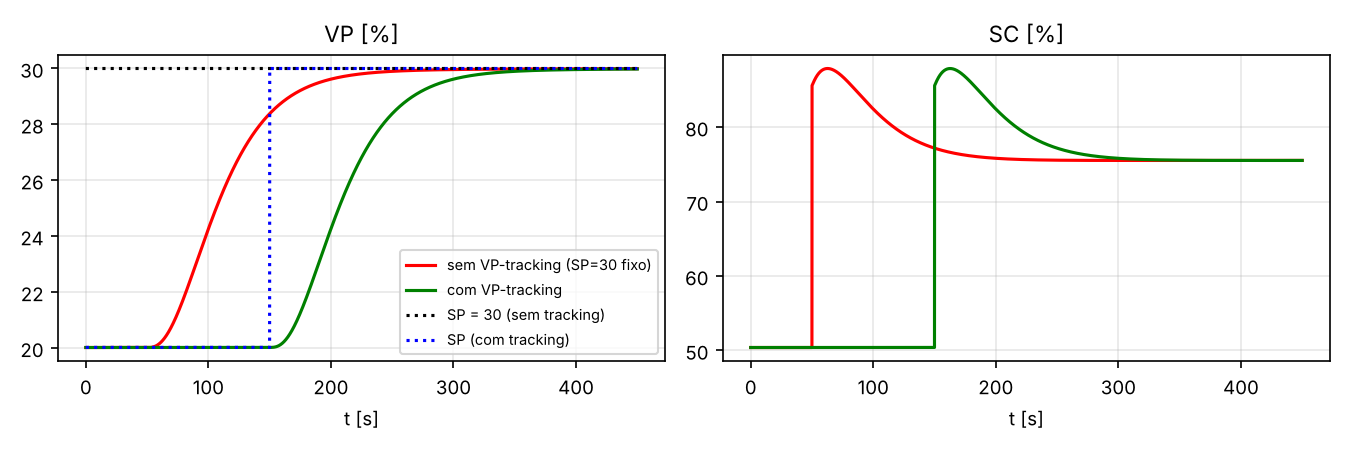
\includegraphics[width=.95\textwidth]{figs/g12.png}\end{figure}
Parte A: no instante da transferência o SC salta de $50{,}4$ para $\approx85{,}6\,\%$ ($=50{,}4+3{,}523\cdot(30-20)$) e a VP sobe imediatamente, sem que o operador tenha dado ``ordem de degrau''. Parte B: o SC fica em $50{,}4\,\%$ na transferência; o degrau de SP depois produz a resposta normal.\end{esp}
\begin{dica}O salto observado depende de como o bloco inicializa o integrador (aqui supus que o integrador assume o valor do SC manual). Se o seu bloco zerar o integrador, o SC pode \emph{cair} ($\approx K_p\cdot e=35\,\%$) em vez de subir; descreva o que viu e explique: em ambos os casos há um \emph{bump} indesejado.\end{dica}
\textbf{O que gravar:} SO, SP, VP em ambas as partes. \textbf{O que concluir:} sem tracking há um salto $=K_p(SP-VP)$ no SC (bump); com tracking, a transferência é suave.

\begin{real}\textbf{Q12 (seu ensaio):} manual com $SO=20\,\%$, $VP=7{,}71$, SP deixado em 0 (sem tracking); operador pôs $SP=16$ e passou a automático em $t=593$ s. O SO saltou de $20$ para $\approx50$ (mediana $50{,}2$ entre 595 e 615 s; previsto $20+3{,}523\cdot8{,}29=49{,}2$). A VP subiu imediatamente (RMS $\times$ simulação $=0{,}24\,\%$). Na Q11 (com tracking, $SP=VP$) o SO continuou em $\approx50$: sem salto.\end{real}

\subsection{Item 1.3 --- Problema sem anti reset windup (seção 5-3.4)}
\textbf{Ideia.} Pedir um SP \emph{inalcançável} (acima de $K_3\cdot100\approx39{,}2\,\%$): o SC satura em 100\,\%, o erro persiste e o integrador acumula. Quando o SP volta a um valor alcançável, o integrador está ``carregado'' e a VP demora a responder.
\begin{parm}Sintonia do 1.1. Sequência de SP: \textbf{25\,\% (regime)} $\to$ \textbf{45\,\%} (por $\sim$300 s) $\to$ \textbf{30\,\%}. SC saturado em 0--100\,\%.\end{parm}
\textbf{Passo a passo:}
\begin{enumerate}
\item Manual: $SO=25/0{,}3918=63{,}8\,\%$ por 8 min ($VP\to25\,\%$). Parâmetros do 1.1. SC com saturação em 0--100\,\% (confirme).
\item \textbf{Versão sem anti-windup:} desative o \texttt{STOP\_INTGR} (Seção~\ref{editarst}: \texttt{STOP\_INTGR := FALSE}). Automático com $SP=25$.
\item Após 50 s: $SP=45\,\%$. Mantenha \textbf{300 s} (SC fica em 100\,\%; VP estaciona em $\approx39$\,\%). Anote o horário.
\item Mude para $SP=30\,\%$. Observe e grave até a VP chegar a 30\,\% ($\sim$10 min).
\item \textbf{Versão com anti-windup:} (repita a condição inicial) repita a sequência com o programa original (\texttt{STOP\_INTGR} ligado).
\end{enumerate}
\begin{esp}\begin{figure}[H]\centering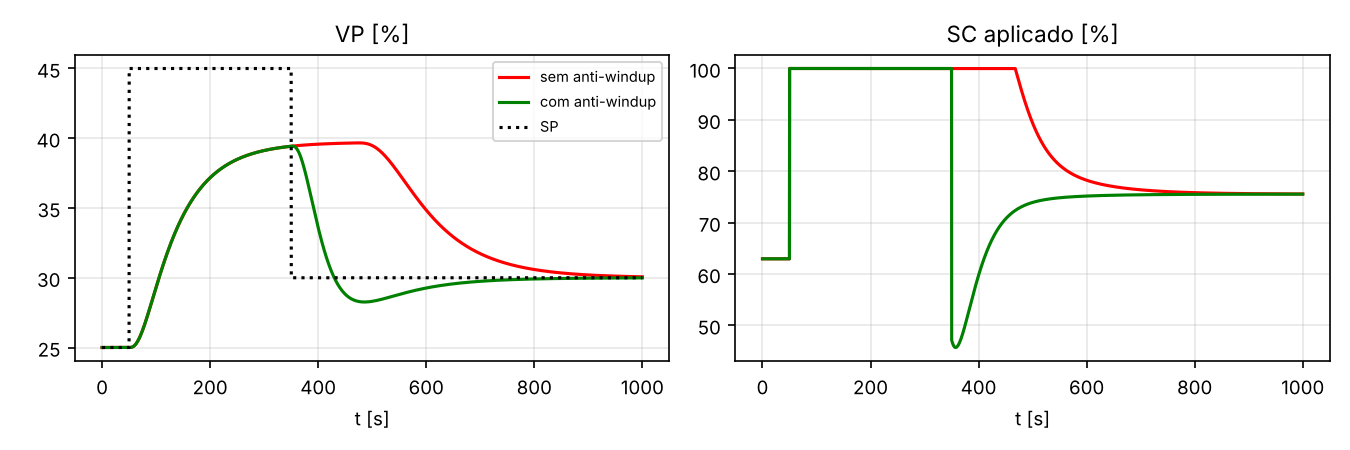
\includegraphics[width=.95\textwidth]{figs/g13.png}\end{figure}
Sem anti-windup: depois do SP voltar a 30\,\%, o SC \emph{continua em 100\,\%} e a VP fica em $\approx39{,}5\,\%$ por mais de 100 s; só chega a $\pm0{,}5$ de 30\,\% cerca de \textbf{465 s} depois da mudança. Com anti-windup: o SC desce imediatamente e a VP chega a 30\,\% em $\approx$\textbf{74 s} (com um pequeno subsinal). (O tempo de recuperação sem proteção cresce com o tempo em que o SP ficou inalcançável.)\end{esp}
\textbf{O que gravar:} SO (SC), SP e VP nas duas versões. \textbf{O que concluir:} windup = integrador acumulando durante a saturação; o atraso na saída da saturação.

\begin{real}\textbf{Q13a (sem AW) e Q13b (com AW):} SP 55 (inalcançável por 449 s e 501 s) e depois 20. Sem anti-windup o SO ficou \textbf{337 s} em 99,94\,\% depois da queda do SP, a VP ficou em 39,3\,\% por $\approx340$ s e só chegou a $20\pm1\,\%$ em $\approx700$ s. Com anti-windup o SO saiu da saturação \textbf{imediatamente}, a VP começou a cair em 13 s (dinâmica da planta) e chegou a $20\pm1\,\%$ em 123 s. \textbf{Conta para explicar:} integral acumulada $\approx414$ pontos; para sair da saturação precisa $I<99{,}94-K_pe=99{,}94+68=168$; desce $K_i|e|=0{,}03872\cdot19{,}3=0{,}75$ ponto/s $\Rightarrow(414-168)/0{,}75=328$ s (medido: 337 s).\end{real}

\subsection{Item 2.1 --- PID 2GL ($\alpha_{TCC}=0{,}64\Rightarrow$ \texttt{alfa := 0.36})}
\begin{parm}$K_p=5{,}057$;\ $K_i=0{,}05558$ ($T_i=90{,}99$);\ $K_d=56{,}21$ ($T_d=11{,}11$);\ \textbf{\texttt{alfa := 0.36}} ($=1-0{,}64$; \textbf{não digite 0,64}).\quad Degrau de SP: \textbf{20 $\to$ 30\,\%}.\end{parm}
\textbf{Passo a passo:} procedimento comum com \texttt{alfa := 0.36}. Se possível, repita depois com \texttt{alfa := 1.0} (PI\_D comum).
\begin{esp}\begin{figure}[H]\centering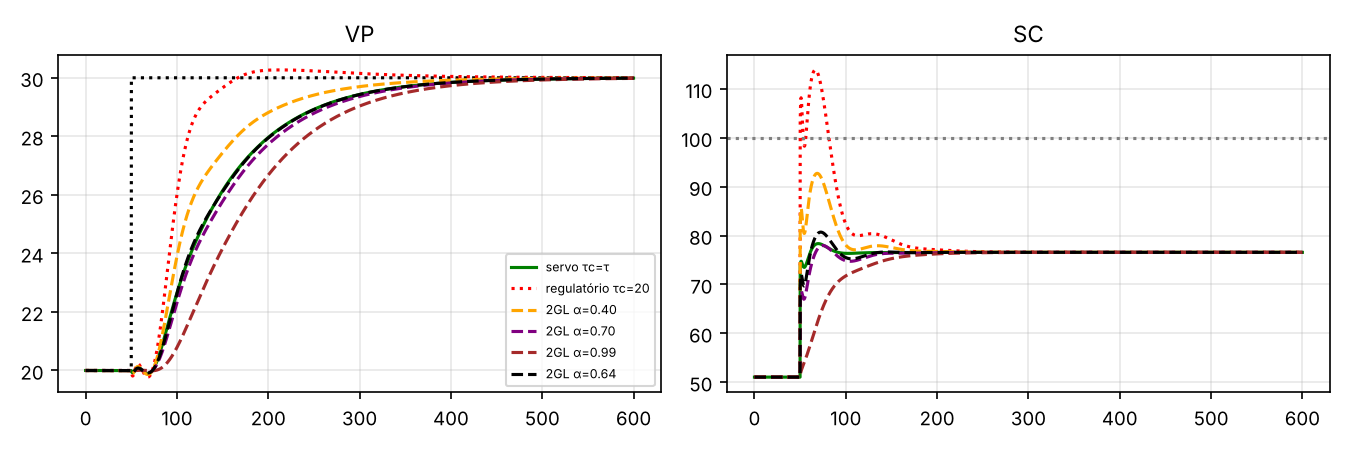
\includegraphics[width=.95\textwidth]{figs/i21.png}\end{figure}
Com $\alpha_{TCC}=0{,}64$ (\texttt{alfa}$=0{,}36$): sem sobressinal, $t_{63,2}\approx103$--105 s, $t_s\approx330$--350 s, pico do SC $\approx$\textbf{75--81\,\%}. Com $\alpha_{TCC}=0$ (\texttt{alfa}$=1$, regulatório): sobressinal $\approx2{,}5\,\%$, $t_{63,2}\approx52$ s, SC chegando a \textbf{103--114\,\%} (saturaria). SC final $\approx75{,}5$--76,6\,\%.\end{esp}
\textbf{Conclusão a escrever:} o $\alpha$ suaviza o SC e reproduz a resposta servo mantendo o ganho regulatório.

\subsection{Item 2.2 --- Distúrbio com $R_p$ (válvula 50\,\%)}
\textbf{Ideia.} $R_p$ em paralelo com $C_3$ (nó 3 $\to$ terra) é uma válvula de escoamento extra. Metade da capacidade da válvula $R_4$ $\Rightarrow$ $R_p=2R_4=133{,}6$ k$\Omega$ (condutância $g_p=7{,}49\ \mu$S).
\begin{alerta}O enunciado diz ``uma das válvulas''. Escolhi a de saída ($R_4$) por ser a que tem o efeito de ``abrir o dreno'' do último tanque; \textbf{confirme com o professor} qual válvula ele quer analogamente. Se for outra, recalcule $R_p=2R_k$ e refaça a simulação com \texttt{--rp}.\end{alerta}
\textbf{Efeito no modelo.} O ganho cai para $K_3'=0{,}3052$ ($-23\,\%$): em malha aberta a VP iria de 25 para $0{,}3052\cdot62{,}9=19{,}2\,\%$; em malha fechada o controlador precisa subir o SC de $62{,}9$ para $25/0{,}3052=81{,}9\,\%$.
\begin{parm}Sintonia do 2.1 ($K_p=5{,}057$, $T_i=90{,}99$, $T_d=11{,}11$). $SP=25\,\%$ constante (sem degrau de SP).\end{parm}
\textbf{Passo a passo:}
\begin{enumerate}
\item Manual: $SO=25/0{,}3918=63{,}8\,\%$ por 8 min. Automático com $SP=25\,\%$ (=VP). Grave 100 s para ter linha de base.
\item Prepare $R_p$ (133,6 k$\Omega$) com um fio solto num lado e o outro lado no terra.
\item \textbf{Ligue $R_p$} entre o nó 3 e o terra (anote o horário exato). \textbf{Não toque no SP.}
\item Grave até a VP voltar a 25\,\% ($\sim$300 s). Opcional: desligue $R_p$ e observe o distúrbio inverso.
\item Opcional para comparar: repita com a sintonia \emph{servo} ($K_p=2{,}234$, $K_i=0{,}02455$, $K_d=24{,}83$) para mostrar que a regulatória rejeita melhor.
\end{enumerate}
\begin{esp}\begin{figure}[H]\centering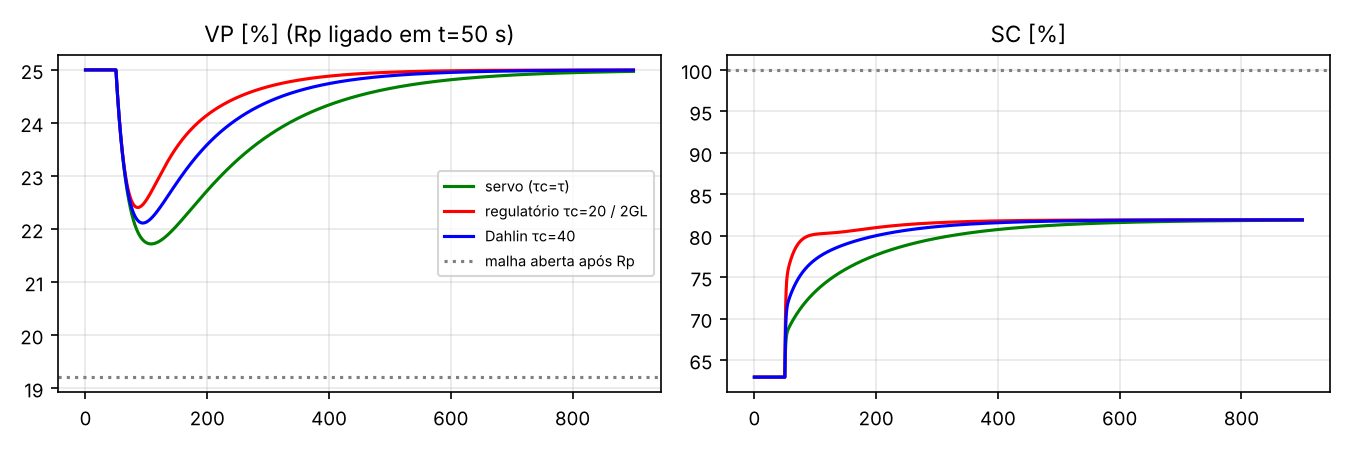
\includegraphics[width=.95\textwidth]{figs/g22.png}\end{figure}
VP cai $\approx$\textbf{2,6 pontos} (regulatório) e volta a $\pm1$ em $\approx$\textbf{134 s}; servo cai $3{,}3$ e leva $\approx284$ s; Dahlin ($\tau_c=40$) cai $2{,}9$ e leva $\approx190$ s. SC sobe até $\approx$\textbf{81,9\,\%} e estabiliza. O $\alpha$ \textbf{não} altera esta resposta ($VP/D$ não contém $C_f$).\end{esp}
\textbf{Simulação para o relatório:} use o script com \texttt{--rp 133600 --rp-t <instante do $R_p$>} (Seção~\ref{pos}).

\subsection{Item 3.1 --- Integral do erro mínimo (seção 7-2.3)}
\begin{parm}$K_p=7{,}222$;\ $K_i=0{,}06449$ ($T_i=111{,}98$);\ $K_d=71{,}63$ ($T_d=9{,}92$);\ $\mu=0{,}1$.\quad Degrau de SP: \textbf{20 $\to$ 25\,\%}.\end{parm}
\textbf{Passo a passo:} procedimento comum, com $SO_0=51{,}0\,\%$.
\begin{esp}\begin{figure}[H]\centering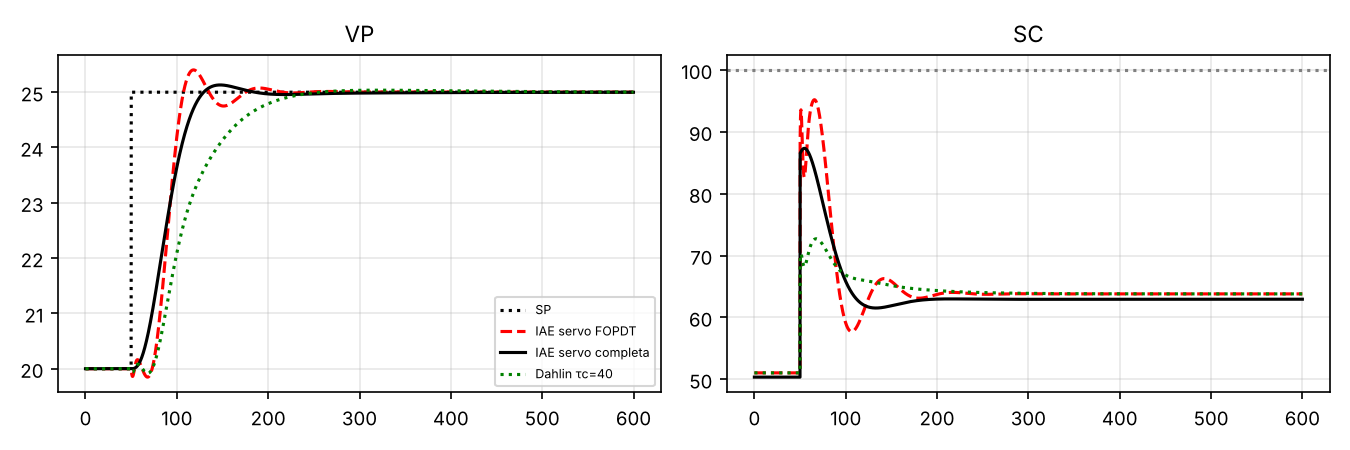
\includegraphics[width=.95\textwidth]{figs/i31.png}\end{figure}
Sobressinal $\approx$ \textbf{2,6\,\%} (FT completa; $8{,}1\,\%$ na FOPDT); $t_{63,2}\approx44$ s; acomodação $\approx110$--117 s; pico do SC 87--95\,\%; SC final $\approx63$\,\%. É \emph{mais rápida} que a Dahlin do 1.1 ($t_{63}=68$ s), com mais sobressinal.\end{esp}
\begin{alerta}Com este ganho, degrau de 20 $\to$ 30\,\% saturaria o SC. Mantenha 20 $\to$ 25\,\%.\end{alerta}

\subsection{Item 4.1 --- Ziegler--Nichols 1/4 (Tabela 7-1.1)}
\textbf{Parte 1 --- teste de ganho final (experimental):}
\begin{enumerate}
\item Condição inicial: $SP_0=10\,\%$ ($SO=10/0{,}3918=25{,}5\,\%$), 8 min. Escolher um ponto de operação baixo deixa folga para o SC oscilar.
\item Controlador \textbf{só proporcional}: $K_i=0$, $K_d=0$ (ou $T_i$ muito grande e $T_d=0$). Comece com $K_c=15$.
\item Automático. Aplique degrau de SP de $+2$ pontos. Observe a oscilação.
\item Aumente $K_c$ em passos de $\sim$5 (depois 2, depois 1) até a VP oscilar com amplitude \textbf{constante}. Esse é o $K_{cu}$. Meça o período entre picos (=$T_u$) no gráfico (use vários picos).
\item \textbf{Cuidado:} com $K_c$ alto o SC satura (0--100\,\%); procure o \emph{menor} $K_c$ que sustenta a oscilação sem estar saturado de forma crítica (reduza o degrau de SP se necessário).
\end{enumerate}
\begin{esp}Esperado (FT completa): $K_{cu}\approx39$ e $T_u\approx68{,}9$ s ($\omega_u=0{,}091$ rad/s). Valores medidos tipicamente ficam 5--15\,\% diferentes (K real, ADC, atraso do scan do PLC). Com $0{,}5K_{cu}$ a oscilação amortece; com $1{,}2K_{cu}$ ela cresce.\begin{figure}[H]\centering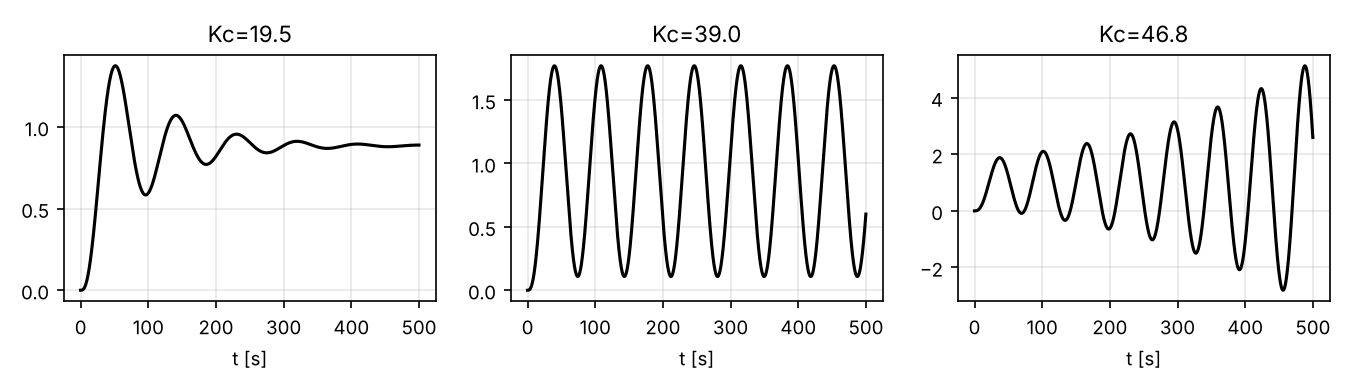
\includegraphics[width=.9\textwidth]{figs/i41_kcu.png}\end{figure}\end{esp}
\textbf{Parte 2 --- PID de Z--N:} recalcule com os \emph{seus} $K_{cu}$ e $T_u$:
\[K_p=0{,}735K_{cu},\quad T_i=0{,}625T_u,\quad T_d=0{,}1T_u,\quad K_i=K_p/T_i,\quad K_d=K_pT_d .\]
Com os valores da simulação: $K_p=28{,}65$; $T_i=43{,}03$; $T_d=6{,}885$; $K_i=0{,}6659$; $K_d=197{,}3$. Degrau de SP \textbf{10 $\to$ 12\,\%}.
\begin{esp}\begin{figure}[H]\centering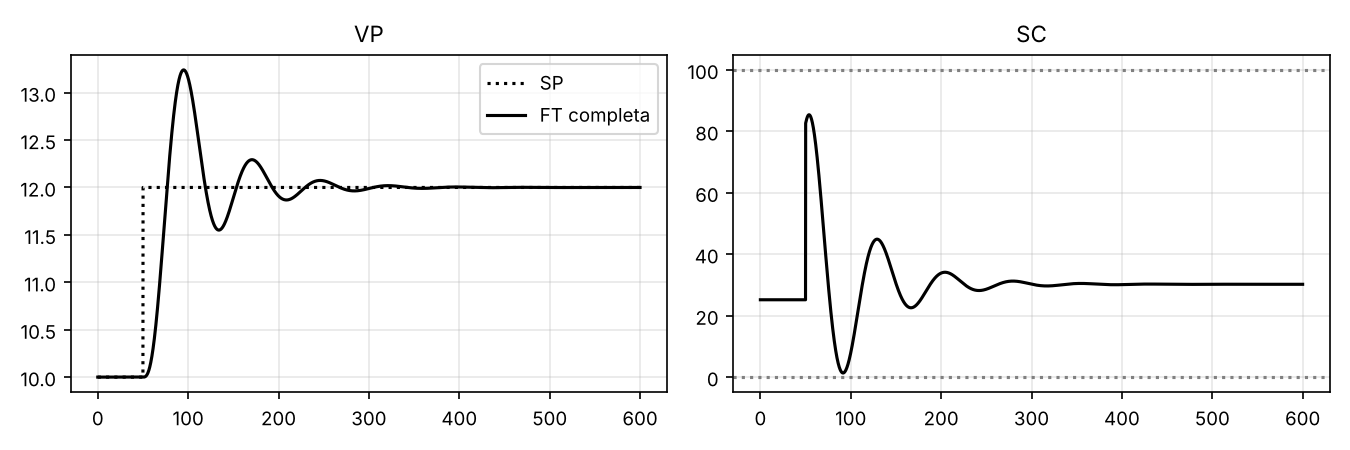
\includegraphics[width=.95\textwidth]{figs/i41.png}\end{figure}
Sobressinal $\approx$\textbf{62--65\,\%} do degrau (VP até $\sim13{,}3\,\%$), $t_{63,2}\approx21$ s, acomodação $\approx209$ s, razão de decaimento $\approx0{,}24$ ($\approx1/4$), SC com pico de $\sim$85\,\% e que \textbf{toca 0\,\%} no primeiro retorno (na bancada vai saturar; diferença esperada em relação à simulação linear).\end{esp}

\subsection{Item 4.2 --- I\_PD com a sintonia do 4.1}
\textbf{Ideia.} Usar os \emph{mesmos} $K_p$, $K_i$, $K_d$ do 4.1, mas com a estrutura I\_PD (só o integrador atua sobre o erro; P e D atuam sobre a VP). No OpenPLC isso é uma opção do bloco (confirme).
\begin{parm}$K_p=28{,}65$;\ $K_i=0{,}6659$;\ $K_d=197{,}3$;\ modo \textbf{I\_PD} $=$ \textbf{\texttt{alfa := 0.0}} no programa (P e D sobre a VP; só a integral sobre o erro).\quad Degrau de SP: \textbf{10 $\to$ 12\,\%}.\end{parm}
\textbf{Passo a passo:} procedimento comum (condição inicial $SO_0=25{,}5\,\%$); selecione I\_PD; degrau de SP 10 $\to$ 12\,\%; grave. Se houver tempo, repita com a estrutura PI\_D (item 4.1) para sobrepor.
\begin{esp}\begin{figure}[H]\centering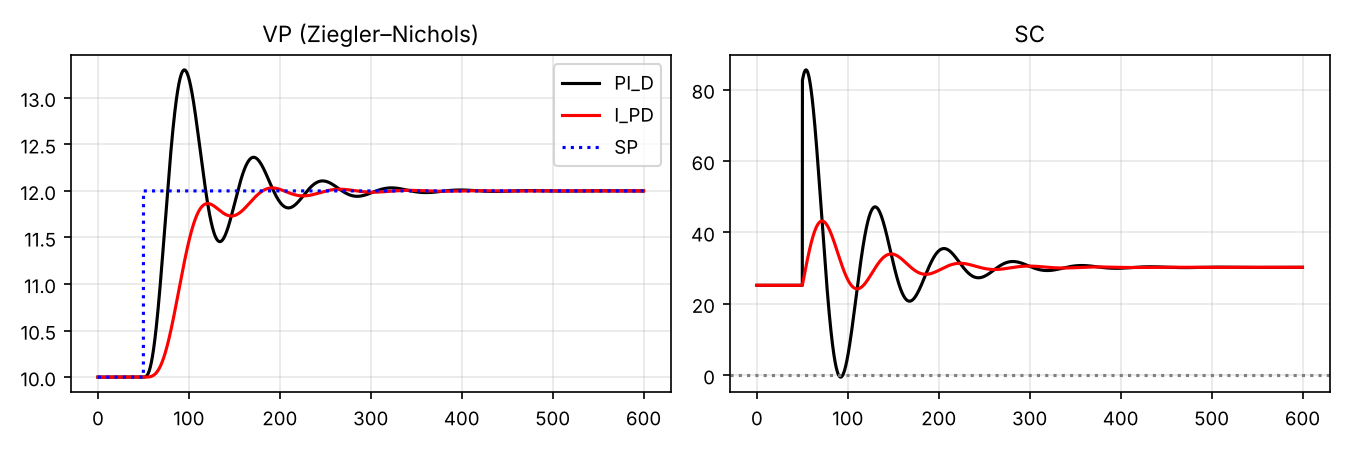
\includegraphics[width=.95\textwidth]{figs/g42.png}\end{figure}
PI\_D: sobressinal $\approx65\,\%$, $t_{63}\approx21$ s, SC pula $\approx+57$ pontos (pico $\sim$85\,\%). I\_PD: sobressinal $\approx$\textbf{1,6\,\%}, $t_{63}\approx$\textbf{46 s} (mais lento), \textbf{sem salto no SC} (pico $\sim$43\,\%, mínimo $\sim$24\,\%).\end{esp}
\textbf{Explicação para o relatório:} em I\_PD a FT de SP para VP é $\dfrac{K_i\,G}{1+(PI+D)G}$ (só $K_i$ no numerador): o zero do PI (que causa o sobressinal e o salto do SC) desaparece. O polinômio característico é o mesmo, então a \emph{rejeição de distúrbio} não muda, mas o seguimento de SP fica suave e mais lento. É útil quando o ganho é alto e o atuador é sensível a degraus de SP.

%--------------------------------------------------------------------
\section{Pós-processamento e comparação com a simulação}\label{pos}
\subsection{Exportar e preparar o CSV}
\begin{enumerate}
\item Gere o relatório CSV no ScadaBR (período do ensaio, aquisição 1 s).
\item O CSV real do ScadaBR é em formato ``longo'' (\texttt{Nome do data point, Tempo, Valor, \ldots}) e \textbf{cada variável tem um número diferente de linhas} (ex.: SO 2024, VP 2028). Por isso \textbf{não se pode dividir o arquivo por 5} como no script de exemplo do professor: os scripts desta pasta separam as variáveis pelo \emph{nome} e alinham numa grade de 1 s.
\item Defina onde começa o trecho a comparar (use o parâmetro \texttt{--inicio} para cortar o período em manual). A simulação assume que no \textbf{primeiro ponto do trecho} a planta está em regime com $SC=SO(1)$.
\end{enumerate}
\subsection{Script em Python (testado) --- \texttt{simula\_bancada.py}}
Simula a \textbf{FT completa} em malha fechada com o PI\_D paralelo (derivada na VP, filtro $\mu$), com opções de $\alpha$ (2GL), I\_PD, saturação, anti-windup por \emph{clamping} e $R_p$.
\begin{lstlisting}
# Teste interno (deve imprimir pico de SC ~88 e sobressinal do Z-N ~62-65):
python3 simula_bancada.py autoteste

# Item 1.1 (comparar com a bancada; --inicio corta amostras iniciais):
python3 simula_bancada.py comparar MEUARQUIVO.csv --kp 3.523 --ti 90.99 --td 11.114

# Item 2.1:   --kp 5.057 --ti 90.99 --td 11.114 --alpha 0.64
# Item 2.2:   --kp 5.057 --ti 90.99 --td 11.114 --rp 133600 --rp-t 100   (rp-t = segundo do trecho em que ligou o Rp)
# Item 3.1:   --kp 7.222 --ti 111.98 --td 9.917
# Item 4.1:   --kp 28.654 --ti 43.031 --td 6.885 --sat
# Item 4.2:   --kp 28.654 --ti 43.031 --td 6.885 --modo I_PD --sat
# Item 1.3:   --kp 3.523 --ti 90.99 --td 11.114 --sat --aw none (Q13a)  |  --aw clamp (Q13b)
# Exemplo real: python3 simula_bancada.py comparar Q11.csv --inicio 1605 --kp 3.523 --ti 90.99 --td 11.114 --sat --aw clamp
\end{lstlisting}
A saída traz o \textbf{RMS e o erro máximo} de VP e de SC e salva \texttt{comparacao.png} (VP exp.\ $\times$ sim.\ e SC exp.\ $\times$ sim.). \textbf{Edite $R$ e $C$ no topo do arquivo} se os seus valores medidos forem outros.
\begin{alerta}A leitura do CSV foi \textbf{testada com os seus arquivos reais} (Q11, Q12, Q13a, Q13b). Use \texttt{--sat} para aplicar os limites reais do SC (10 e 99,94\,\%; mudam com \texttt{--umin/--umax}) e \texttt{--aw clamp} ou \texttt{--aw none} para o anti-windup. O SC experimental é muito ruidoso: o script compara o SC simulado com a \textbf{mediana móvel} do SO (e mostra também o RMS do SO bruto). Em 1.2 (bumpless) a simulação com \texttt{--inicio} no instante da transferência reproduz o salto.\end{alerta}
\subsection{Script MATLAB --- \texttt{compara\_malha.m} (estilo do professor)}
Mesma lógica (planta completa, simulação discreta). \textbf{Não foi executado no MATLAB} (não disponível aqui); a lógica é a do Python acima. Teste primeiro com o caso 1.1 e confira se a simulação dá pico de SC $\approx88\,\%$.
\begin{lstlisting}
% Edite no topo: arquivo, inicio, R, C, Kp, Ti, Td, mu, alpha, modo, umin/umax, aw, Rp, tRp.
% A leitura usa o formato REAL do ScadaBR (separa as variaveis pelo nome do ponto, grade de 1 s).
T=readtable(arquivo,'Delimiter',',','Encoding','ISO-8859-1','VariableNamingRule','preserve','DecimalSeparator','.');
nomes=strtrim(string(T{:,1})); tempo=datetime(string(T{:,2}),'InputFormat','yyyy/MM/dd HH:mm:ss'); valor=T{:,3};
SO=serie(nomes,tempo,valor,'SO'); SP=serie(nomes,tempo,valor,'SP'); VP=serie(nomes,tempo,valor,'VP');
% ... (ver scripts/compara_malha.m: simulacao discreta + graficos + RMS)
\end{lstlisting}
\subsection{Diferenças entre o script do professor e o meu}
\begin{itemize}
\item O do professor usa \textbf{PID = P+I+D com derivada no erro} (\texttt{PID=P+I+D}); o OpenPLC é \textbf{PI\_D} (derivada na VP). Os scripts deste guia usam a forma do OpenPLC.
\item O do professor usa Padé de 1ª ordem para o atraso e a FOPDT; aqui uso a \textbf{planta completa} (sem Padé). Para comparar com a FOPDT, use a Resolução (Padé de 3ª ordem).
\item O do professor simula em \textbf{desvios} (\texttt{SP-SP(1,1)}); meus scripts usam \textbf{valores absolutos} ($SC_0=SO(1)$). Ao comparar com o dele, desloque o SC.
\end{itemize}
\subsection{O que escrever no relatório (para cada item)}
\begin{enumerate}
\item Parâmetros usados; degrau; condições iniciais.
\item Figura VP exp.\ $\times$ sim.\ e SC exp.\ $\times$ sim.
\item \textbf{RMS e erro máximo} de VP e de SC (% da escala).
\item Comentário curto: quais características concordam (tempo de subida, sobressinal, pico do SC, valor final) e \textbf{por que} diferem (K 1,3\,\% menor; ADC 0,098\,\%; saturação do SC; atraso de scan; tolerâncias).
\end{enumerate}

\section{Tabela de resultados esperados (cola de bancada)}
\begin{center}\small
\begin{tabular}{llp{8cm}}\toprule Item & Degrau/ação & Resultado esperado (simulação, FT completa)\\\midrule
1.1 & SP 20$\to$30 & sobress.\ $\le0{,}7\,\%$; $t_{63}\approx70$ s; SC pulo $+35$, pico 88--94, final 75,5\\
1.2 & trocar p/ auto com SP$\ne$VP & SC salta $K_p(SP-VP)\approx35$ pontos (50,4$\to$85,6)\\
1.3 & SP 25$\to$45$\to$30 & sem AW: VP presa em $\approx39{,}5$ por $>100$ s, volta só após $\approx465$ s; com AW: 74 s\\
2.1 & SP 20$\to$30, \texttt{alfa}$=0{,}36$ & sem sobress.; $t_{63}\approx104$ s; pico SC 76--81\\
2.2 & $R_p=133{,}6$ k$\Omega$ ligado & queda 2,6 pontos; recupera em $\approx134$ s; SC final 81,9\\
3.1 & SP 20$\to$25 & sobress.\ $\approx2{,}6\,\%$; $t_{63}\approx44$ s; SC pico 87\\
4.1 & SP 10$\to$12 & sobress.\ 62--65\,\%; $t_{63}\approx21$ s; razão 1/4; SC toca 0\\
4.2 & I\_PD, SP 10$\to$12 & sobress.\ $\approx1{,}6\,\%$; $t_{63}\approx46$ s; sem salto no SC\\\bottomrule\end{tabular}\end{center}

\section{Solução de problemas}
\begin{center}\small
\begin{tabular}{p{4.6cm}p{10.4cm}}\toprule Sintoma & Causa provável / o que fazer\\\midrule
VP$\approx0$ com SO alto & Terra não comum; entrada analógica no pino errado; capacitor com polaridade invertida.\\
VP saturada em 100\,\% ou valores absurdos & Escala errada (0--1023 em vez de \%); ou mapeamento de pino trocado.\\
Ruído de $\pm0{,}1$--0,2\,\% na VP & Normal (ADC 0,098\,\%); em Z--N o $K_d$ alto amplifica; confira $\mu$ e o aterramento.\\
SO pula entre $\approx10$ e $\approx99{,}9\,\%$ com a VP suave & \textbf{Ruído de quantização amplificado pela derivada} (Seção~\ref{licoes}). Teste com $K_d=0$ (PI). Não é instabilidade da malha.\\
SC ``treme'' muito (3.1, 4.1) & Ganho de alta frequência $K_p(1+1/\mu)$; use os valores da tabela; não aumente $K_d$.\\
Resposta mais lenta/rápida que a simulação em $\sim$5--10\,\% & Tolerância de $R$, $C$; $K$ real $\ne$ teórico. Refaça a simulação com os valores medidos.\\
Oscilação em 1.1/2.1/3.1 & $K_i$ ou $K_d$ digitados errado; o bloco usa $T_i$ em vez de $K_i$ (ou o contrário).\\
SC satura onde a simulação não satura & Degrau maior que o do roteiro; ponto inicial diferente (SC$_0$ errado); $K$ diferente.\\
Não repete o experimento & Capacitores não descarregados/regime não atingido; espere 8 min antes do degrau.\\
Tempos do ScadaBR irregulares & Verifique período de atualização (1 s) e carga da CPU; o simulador assume 1 amostra/s.\\\bottomrule\end{tabular}\end{center}

\section{Folha de registro (imprima e preencha)}
\begin{center}\small
\begin{tabular}{|p{5.2cm}|p{9.5cm}|}\hline
Data / hora / sorteio (questão e item) & \\\hline
$R_1,R_2,R_3,R_4$ medidos [k$\Omega$] & \\\hline
$C_1,C_2,C_3$ medidos [$\mu$F] & \\\hline
$K$ medido ($V_{c3}/V_{in}$ em regime) & \\\hline
Parâmetros digitados ($K_p,K_i,K_d,\mu,\alpha$) & \\\hline
Estrutura (PI\_D / 2GL / I\_PD); saturação; anti-windup; tracking & \\\hline
$SP_0$; $SO_0$ inicial; tempo em regime antes do degrau & \\\hline
Instantes das ações (degrau de SP, $R_p$, auto/manual) & \\\hline
Nome do arquivo CSV & \\\hline
RMS VP / RMS SC; erro máx.\ VP / SC & \\\hline
Observações (saturação, ruído, diferenças) & \\\hline
\end{tabular}\end{center}

\section{Roteiro do dia da avaliação}
\begin{enumerate}
\item \textbf{Sorteio.} Anote questão e item; localize no relatório os parâmetros (Seção~\ref{tabpar}).
\item \textbf{Em paralelo:} monte o circuito e já deixe o sistema em manual com $SO=SP_0/K$ (8 min).
\item Confira $R$, $C$ rapidamente (se mudou o circuito, avise e recalcule).
\item Digite os parâmetros; \textbf{releia}. Siga a Seção~\ref{comum}.
\item Grave; exporte; rode o script; mostre VP e SC exp.\ $\times$ sim.
\item \textbf{Esteja pronta para explicar}: de onde vêm as fórmulas (Parte I), por que o SC salta $K_p\Delta SP$, o que muda se $\tau_c$ ou $\alpha$ mudarem, por que a FOPDT é conservadora.
\item Se algo falhar: descreva a causa e diga como corrigiria (a possibilidade de refazer existe).
\end{enumerate}
\end{document}
